% latex uft-8
\documentclass[uplatex,a4paper,11pt,oneside,openany]{jsbook}
%
\usepackage[dvipdfmx]{graphicx}
\usepackage[dvipdfmx]{color}
\usepackage{amsmath,amssymb}
\usepackage{enumerate}
\usepackage{bm}
\usepackage{comment}
\usepackage{ascmac}
\usepackage{setspace}
\usepackage{here}
\usepackage{listings,jlisting} %日本語のコメントアウトをする場合jlistingが必要

\usepackage{xcolor}

\definecolor{mygreen}{rgb}{0,0.6,0}
\definecolor{mygray}{rgb}{0.5,0.5,0.5}
\definecolor{mymauve}{rgb}{0.58,0,0.82}

\begin{comment}
\lstset{
  backgroundcolor=\color{white},   % choose the background color; you must add \usepackage{color} or \usepackage{xcolor}; should come as last argument
  basicstyle=\footnotesize,        % the size of the fonts that are used for the code
  breakatwhitespace=false,         % sets if automatic breaks should only happen at whitespace
  breaklines=true,                 % sets automatic line breaking
  captionpos=b,                    % sets the caption-position to bottom
  commentstyle=\color{mygreen},    % comment style
  deletekeywords={...},            % if you want to delete keywords from the given language
  escapeinside={\%*}{*)},          % if you want to add LaTeX within your code
  extendedchars=true,              % lets you use non-ASCII characters; for 8-bits encodings only, does not work with UTF-8
  firstnumber=1000,                % start line enumeration with line 1000
  frame=single,	                   % adds a frame around the code
  keepspaces=true,                 % keeps spaces in text, useful for keeping indentation of code (possibly needs columns=flexible)
  keywordstyle=\color{blue},       % keyword style
  language=Octave,                 % the language of the code
  morekeywords={*,...},            % if you want to add more keywords to the set
  numbers=left,                    % where to put the line-numbers; possible values are (none, left, right)
  numbersep=5pt,                   % how far the line-numbers are from the code
  numberstyle=\tiny\color{mygray}, % the style that is used for the line-numbers
  rulecolor=\color{black},         % if not set, the frame-color may be changed on line-breaks within not-black text (e.g. comments (green here))
  showspaces=false,                % show spaces everywhere adding particular underscores; it overrides 'showstringspaces'
  showstringspaces=false,          % underline spaces within strings only
  showtabs=false,                  % show tabs within strings adding particular underscores
  stepnumber=2,                    % the step between two line-numbers. If it's 1, each line will be numbered
  stringstyle=\color{mymauve},     % string literal style
  tabsize=2,	                   % sets default tabsize to 2 spaces
  title=\lstname                   % show the filename of files included with \lstinputlisting; also try caption instead of title
}
\end{comment}

%ここからソースコードの表示に関する設定
\lstdefinestyle{customc}{
  belowcaptionskip=1\baselineskip,
  breaklines=true,
  numbers=left,
  frame=none,
  xleftmargin=\parindent,
  language=C,
  showstringspaces=false,
  basicstyle=\footnotesize\ttfamily,
  keywordstyle=\bfseries\color{green!40!black},
  commentstyle=\itshape\color{purple!40!black},
  identifierstyle=\color{blue},
  stringstyle=\color{orange},
}

\lstdefinestyle{custompy}{
    basicstyle={\ttfamily},
    identifierstyle={\small},
    commentstyle={\smallitshape},
    keywordstyle={\small\bfseries},
    ndkeywordstyle={\small},
    stringstyle={\small\ttfamily},
    frame={tb},
    breaklines=true,
    columns=[l]{fullflexible},
    numbers=left,
    xrightmargin=0zw,
    xleftmargin=3zw,
    numberstyle={\scriptsize},
    stepnumber=1,
    numbersep=1zw,
    lineskip=-0.5ex,
    language=Python,
}

\lstdefinestyle{customasm}{
  belowcaptionskip=1\baselineskip,
  frame=L,
  xleftmargin=\parindent,
  language=[x86masm]Assembler,
  basicstyle=\footnotesize\ttfamily,
  commentstyle=\itshape\color{purple!40!black},
}

\lstset{escapechar=@,style=custompy}

\makeatletter
\def\ps@plainfoot{%
  \let\@mkboth\@gobbletwo
  \let\@oddhead\@empty
  \def\@oddfoot{\normalfont\hfil-- \thepage\ --\hfil}%
  \let\@evenhead\@empty
  \let\@evenfoot\@oddfoot}
  \let\ps@plain\ps@plainfoot
\renewcommand{\chapter}{%
  \if@openright\cleardoublepage\else\clearpage\fi
  \global\@topnum\z@
  \secdef\@chapter\@schapter}
\makeatother
%
\newcommand{\maru}[1]{{\ooalign{%
\hfil\hbox{$\bigcirc$}\hfil\crcr%
\hfil\hbox{#1}\hfil}}}
%
\setlength{\textwidth}{\fullwidth}
\setlength{\textheight}{40\baselineskip}
\addtolength{\textheight}{\topskip}
\setlength{\voffset}{-0.55in}
%
\begin{document}
% START DOCUMENT
%
% COVER
\begin{center}
  \huge \par
  \vspace{65mm}
  \huge \par
  \vspace{15mm}
  \LARGE Another Book for Python \par
  \vspace{100mm}
  \Large \today \par
  \vspace{15mm}
  \Large S.Matoike \par
  \vspace{10mm}
  \Large \par
  \vspace{10mm}
\end{center}
\thispagestyle{empty}
\clearpage
\addtocounter{page}{-1}
\newpage
\setcounter{tocdepth}{3}
%
\tableofcontents
%
\chapter{はじめに}
%
\subsubsection{記号の読み方}

\begin{table}[htb]
  \begin{tabular}{|c|l||c|l|} \hline
    記号 & \multicolumn{1}{c||}{読み} & 記号 & \multicolumn{1}{c|}{読み} \\ \hline \hline
    \bf{〜} & ティルダ & \bf{\{} & 中括弧 開く \rule[-6pt]{0pt}{22pt}\\ \hline
    \bf{=} & イコール & \bf{\}} & 中括弧 閉じる \rule[-6pt]{0pt}{22pt}\\ \hline
    \bf{@} & アット・マーク & \bf{[} & 大括弧 開く \rule[-6pt]{0pt}{22pt}\\ \hline
    \bf{\#} & ハッシュ(シャープor井桁) & \bf{]} & 大括弧 閉じる \rule[-6pt]{0pt}{22pt}\\ \hline
    \bf{\$} & ドル・マーク & \bf{\textbar} & バーティカル・バー(縦線) \rule[-6pt]{0pt}{22pt}\\ \hline
    \bf{\%} & パーセント & \bf{!} & エクスクラメーション・マーク(感嘆符) \rule[-6pt]{0pt}{22pt}\\ \hline
    \bf{\textasciicircum} & キャレット & \bf{:} & コロン \rule[-6pt]{0pt}{22pt}\\ \hline
     \bf{\&} & アンパサンド & \bf{;} & セミ・コロン \rule[-6pt]{0pt}{22pt}\\ \hline
    \bf{*} & アスタリスク & \bf{"} & ダブル・プライム(ダブル・クォーテーション・マーク) \rule[-6pt]{0pt}{22pt}\\ \hline
    \bf{(} & 小括弧 開く & \bf{'} & プライム(クォーテーション・マークorアポストロフィ) \rule[-6pt]{0pt}{22pt}\\ \hline
     \bf{)} & 小括弧 閉じる & \bf{\textless} & (AはB)より小さい \rule[-6pt]{0pt}{22pt}\\ \hline
    \bf{_} & アンダー・スコア(下線) & \bf{\textgreater} & (AはB)より大きい \rule[-6pt]{0pt}{22pt}\\ \hline
    \bf{+} & プラス & \bf{.} & ピリオド(小数点) \rule[-6pt]{0pt}{22pt}\\ \hline
    \bf{ー} & ハイフン(マイナス) & \bf{,} & カンマ(コンマ) \rule[-6pt]{0pt}{22pt}\\ \hline
    \bf{\textbackslash}(¥) & バック・スラッシュ(円マーク) & \bf{/} & スラッシュ(フォワード・スラッシュorスラント) \rule[-6pt]{0pt}{22pt}\\ \hline
    \bf{?} & クェスチョン・マーク & \bf{`} & dumb quotes「まぬけな引用符」か?(ほとんど使わない) \rule[-6pt]{0pt}{22pt}\\ \hline
  \end{tabular}
\end{table}

文字コードの歴史的な事情(ASCII コードを元に JIS X 0201 が策定された際に、バック・スラッシュ(\)の文字コードの所に円マーク(¥)が割り当てられた事)により、Windows ではアプリケーションプログラム毎に、その作成者の都合でどちらか一方が表示されるという、ややこしい事になっています。

Windows以外のOS(MacやLinuxなどのUnix系OS)では、どちらの文字もキーボードから入力できるので混乱はありません。
プログラムの編集などではむしろ、バック・スラッシュを表示するのがいいかもしれません。(グローバルに活躍できる技術者を目指すならば、、、)

最近では、UTF-8 などの Unicode と呼ばれる文字コードが主流となり、それが標準となってきていることから、Windowsでも区別して扱えるように対応されつつあります。

\subsubsection{日本語キーボードは不要}

キーボードから直接日本語を入力することはありません

日本語はアルファベットを使ってローマ字で入力し、それを漢字に変換して入力します

キーボードに書かれている日本語の表記は、プログラミング学習では不要です。

キートップの右半分は無視しましょう。\\

また、半角のアルファベットの文字は、
そのままキーを押すと小文字が入力され、

Shiftキーを押しながらキーを押すと大文字を入力できます。

\begin{figure}[H]
  \centering
  \begin{tabular}{ll}
      \begin{minipage}[t]{0.9\hsize}
        \centering
  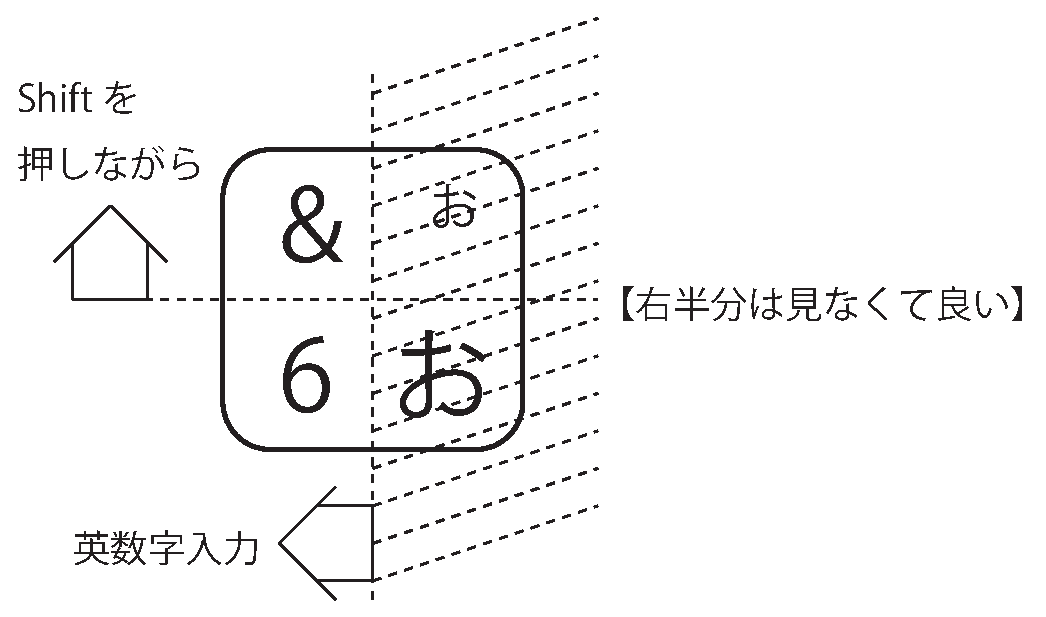
\includegraphics[scale=0.43]{figures/eps/zu2-1.eps}
      \end{minipage}
      \begin{minipage}[t]{0.1\hsize}
      %\centering
      %\begin{equation*}
      %  x = \frac{v-a}{b-a} \times L
      %\end{equation*}
%\includegraphics[scale=0.4]{field.pdf}
      \end{minipage}
    \end{tabular}
\end{figure}%

漢字の全角文字と半角の英数字を、きちんと区別して入力できるようになりましょう。

Pythonでは特に、半角の空白文字による段付け(インデント)が、文法上重要な役目を担っています。

C言語やJavaでは、インデントが不自然でもそのプログラムは動作しましたが、

Pythonでは、インデントがいい加減だと意味不明としてエラーになります。

半角の空白文字が必要なところを全角の空白文字で埋めてしまうと、見た目では判別しづらいのですがプログラムではエラーになってしまいます。


\begin{table}[htb]
  \begin{tabular}{|c|l||c|l|} \hline
    記号 & \multicolumn{1}{c||}{読み} & 記号 & \multicolumn{1}{c|}{読み} \\ \hline \hline
    \bf{〜} &  & \bf{\{} &  \rule[-6pt]{0pt}{22pt}\\ \hline
    \bf{=} &  & \bf{\}} &  \rule[-6pt]{0pt}{22pt}\\ \hline
    \bf{@} &  & \bf{[} &  \rule[-6pt]{0pt}{22pt}\\ \hline
    \bf{\#} & ハッシュ(シャープor井桁) & \bf{]} &  \rule[-6pt]{0pt}{22pt}\\ \hline
    \bf{\$} &  & \bf{\textbar} &  \rule[-6pt]{0pt}{22pt}\\ \hline
    \bf{\%} &  & \bf{!} &  \rule[-6pt]{0pt}{22pt}\\ \hline
    \bf{\textasciicircum} &  & \bf{:} &  \rule[-6pt]{0pt}{22pt}\\ \hline
     \bf{\&} &  & \bf{;} &  \rule[-6pt]{0pt}{22pt}\\ \hline
    \bf{*} &  & \bf{"} &  \rule[-6pt]{0pt}{22pt}\\ \hline
    \bf{(} &  & \bf{'} &  \rule[-6pt]{0pt}{22pt}\\ \hline
     \bf{)} &  & \bf{\textless} & (AはB)より小さい \rule[-6pt]{0pt}{22pt}\\ \hline
    \bf{_} &  & \bf{\textgreater} & (AはB)より大きい \rule[-6pt]{0pt}{22pt}\\ \hline
    \bf{+} &  & \bf{.} &  \rule[-6pt]{0pt}{22pt}\\ \hline
    \bf{ー} &  & \bf{,} &  \rule[-6pt]{0pt}{22pt}\\ \hline
    \bf{\textbackslash}(¥) &  & \bf{/} &  \rule[-6pt]{0pt}{22pt}\\ \hline
    \bf{?} & & \bf{`} & dumb quotes「まぬけな引用符」か?(ほとんど使わない) \rule[-6pt]{0pt}{22pt}\\ \hline
  \end{tabular}
\end{table}

\chapter{変数}

\section{変数}

プログラミングにおける変数とは「プログラムで使うデータを一時的に格納する入れ物」のようなもの

変数には、数値の他、文字列やリスト(値の並び)など、様々なデータを入れられます

変数にデータを格納することを「代入する」といいます

変数に値を代入するには「変数=値」の様に記述し、「=」を「代入演算子」といいます

この時「=の右側(右辺)にある値を、=の左側(左辺)にある変数に代入する」という意味です

「右辺と左辺が等しい」という意味ではありません

Pythonでは変数の型宣言は基本的に必要ないので、変数を使いたいときに値を代入するだけです

C言語やJavaでは変数の型を指定して宣言する必要がありました(静的型付け言語といいます)

\subsubsection{整数型変数}

変数の命名規則(この規則は守らないとエラーになる)
\begin{itemize}
  \item 変数名には半角文字を使う
  \item 変数名は数字から始まらない
  \item アルファベットの大文字、小文字、及び数字とアンダー・スコア(\_)から構成する
  \item アンダー・スコア(\_)から始まる変数名には、Pythonの文法上の意味がある
  \item Pythonの文法上使われる予約語は変数名に使えない
\end{itemize}

変数、定数などの命名に関する暗黙の規則(この規則は紳士協定です)
\begin{itemize}
  \item どのようなデータが格納されているのか、想像しやすい名前を、英単語を基本として命名する
  \item 変数名では、英単語の単語と単語の間をアンダー・スコア(\_)で接続する(snake case)
  \item 定数名には、アルファベットの小文字を含まない名前を使用する
  \item クラス名には、単語と単語の間はつめて、単語の先頭文字を大文字にする(camel case)
\end{itemize}

#の右側には、コメントを記述できます

#によるコメントは独立した行に書くのではなく、Pythonの文の右側に書くようにします
(これは、Pythonのプログラム記述上の紳士協定ですが、本稿では解説する都合に合わせて、
独立した行にコメントを書くことが多いので注意してください)

\lstinputlisting[caption=変数と定数,label=p01-2]{programs/python/p01-2.py}

$a+b$や$a-b$など、2つの項aとbの間の演算を行っているので、2項演算子といいます

C言語やJavaには、$a//b$や$a**b$のような演算子はないので注意しましょう

複合代入演算子(+=や−=)は、代入演算子(=)の操作と共に+やーなどの処理も同時に行う演算子です。
インクリメントの演算$a+=1$ は、 $a = a + 1$と同じ意味です。
%
%\begin{table}[H]
%  \caption{}
%  \label{}
%  \begin{tabular}{l|l}
%    a += b & a = a + b \\
%    a -= b & a = a - b \\
%    a *= b & a = a * b \\
%    a /= b & a = a / b \\
%    a \%= b & a = a \% b \\
%    a //= b & a = a// b \\
%    a **= b & a = a ** b \\
%  \end{tabular}
%\end{table}

\begin{figure}[H]
  \centering
  \begin{tabular}{lr}
      \begin{minipage}{0.45\hsize}
      \centering
\lstinputlisting[caption=代入操作,label=p01-5]{programs/python/p01-5.py}
      \end{minipage}
      \begin{minipage}{0.45\hsize}
      \flushright
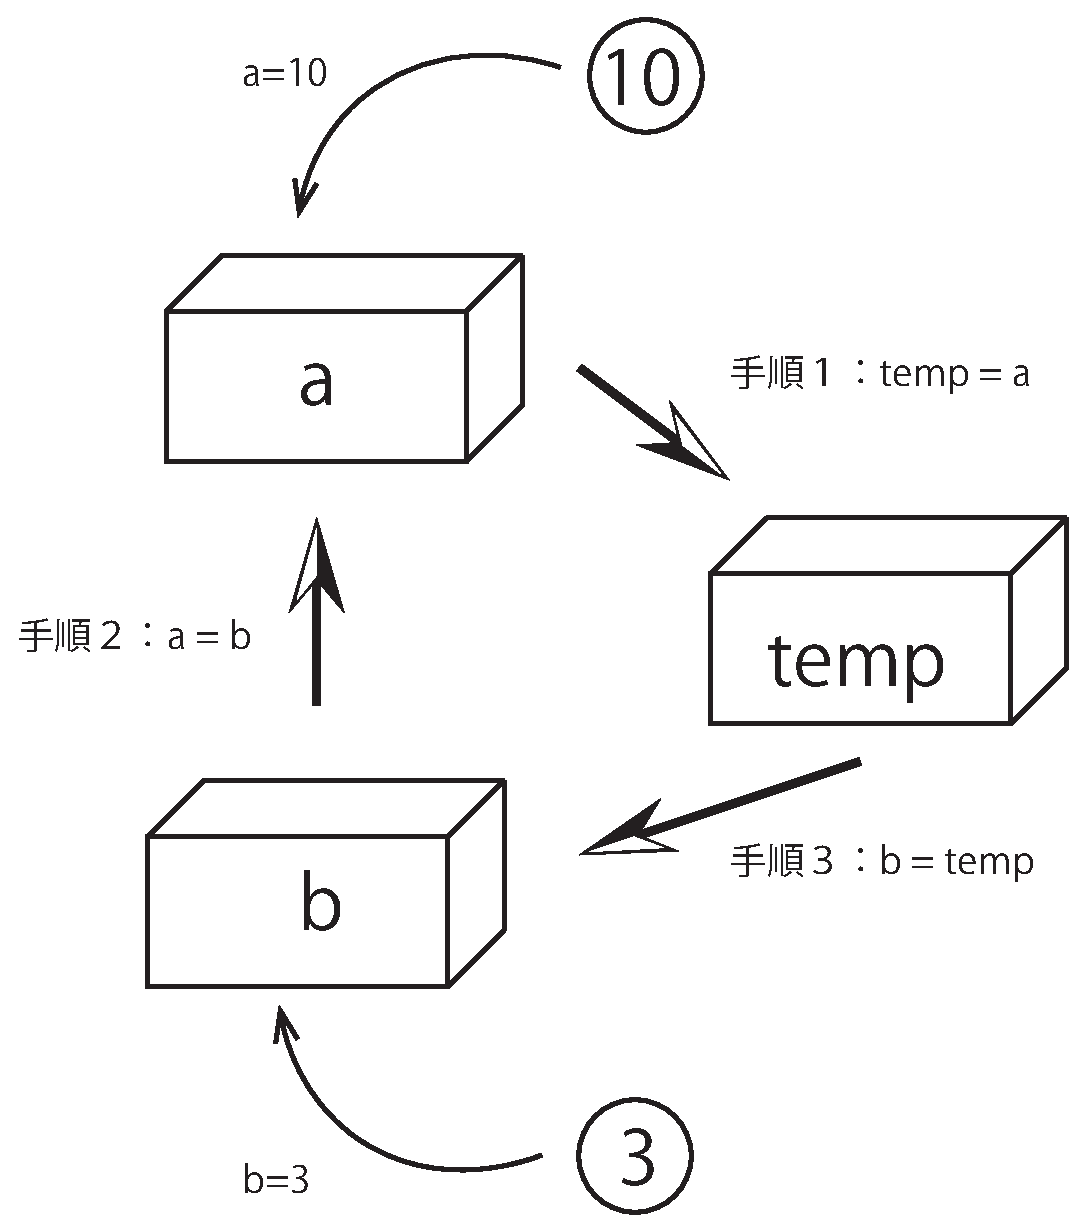
\includegraphics[scale=0.35]{figures/eps/fig1.eps}
      \end{minipage}
    \end{tabular}
\end{figure}%

2つの変数の中身を入れ替える処理はしばしば必要になります

3ステップで行う変数の内容の入れ替え操作についてよく考えて、代入操作について理解して下さい。

なお、
C言語やJavaでは、$a, b = b, a$のように、代入文を1行で書く方法はありません(これはPython独自です)

\subsubsection{文字列型変数}

\lstinputlisting[caption=文字列の変数,label=p01-1]{programs/python/p01-1.py}

文字列はシングル・クォートで挟みます(あるいはダブル・クォートで挟んでもよい)

C言語やJavaにおける文字列は、ダブル・クォートで挟みました

%一方、Pythonでは文字列にシングル・クォートが多用されるので注意しましょう
msgという名前の変数に、"Hello"という文字列をその値として格納しています

print関数を使って、変数msgに格納されている値を表示しています

プラス「+」の演算子によって、文字列を結合することができます

文字列の長さは、len( 文字列 )関数によって得ることができます

%文字列は、リスト(配列)のインデックスを指定して1文字づつ取り出せます

あたかも2文字からなる文字列のように書かれている'$\backslash t$'は、タブ文字と呼ばれる特殊な1文字を表しています

バック・スラッシュの後に1文字を続けて書いて、特殊な機能を持つ1文字を表現する方法を「エスケープ・シーケンス」といいます

タブ文字('$\backslash t$')以外に、改行文字('$\backslash n$')もよく使われます
(C言語のprintf文などで改行文字は多用されています)

\subsubsection{整数、実数と文字列の変換}

数値同士の演算は普通に行えますが、文字列は足したり引いたりと言うわけにはいきません

また、「+」演算子によって文字列同士の連結ができますが、数値を文字列の様に繫ぐことはできません

そこで、以下のようにして変数の型を変換する必要がしばしば生じます

str( 整数型変数 ) によって、整数を文字列に変換できます

str( 実数型変数 ) によって、実数(浮動小数点数)を文字列に変換できます

int( 文字列型変数 ) によって、整数を表す文字列を整数に変換できます

float( 文字列型変数 ) によって、実数を表す文字列を実数(浮動小数点数)に変換できます

\lstinputlisting[caption=キャストによる型の変換,label=p01-4]{programs/python/p01-4.py}

\subsubsection{その他の変数の型}

変数の型を、type関数を使って確認できます

\lstinputlisting[caption=変数の型,label=p01-3]{programs/python/p01-3.py}

\section{標準入出力}

コンピュータには、色々な方法でデータを取り込む(データを入力する)ことができます

例えば、デジカメで撮った画像を取り込んだり、スキャナを使って文書をコンピュータに入力したり

コンピュータへデータを入力する最も手軽な手段は、キーボードから文字を入力することです

キーボードからの入力のことを、「標準入力」という言い方をします(Pythonではinput関数)\\

一方コンピュータは、色々な装置にデータを取り出す(データを出力する)ことができます

例えば、プリンタへ印刷するとか、プロッタに作図するとか、ディスクやDVDに保存するとか

コンピュータからデータを出力する最も身近な装置は、画面(CRTなど)です

画面への出力のことを、「標準出力」といいます(Pythonではprint関数)

\subsection{標準入力}

標準入力(input()関数)では、キーボードからEnterキーが押されるまでコンピュータは待っています

Enterキーを押すまでに叩いた一連のキーを、文字列としてコンピュータに取り込むことになります

%\begin{lstlisting}[basicstyle=\ttfamily\footnotesize,frame=single]
\begin{lstlisting}
# 標準出力へprint()関数を使って、文字列を表示する(出力)
print('メッセージを入力して下さい')
# 標準入力からinput()関数を使って、文字列を受け取る(入力)
str = input()
# 入力した文字列を、確認のため画面に印刷(出力)してみる
print('あなたは、「', str, '」を入力しました')
# 画面にメッセージを出力して、入力操作を促すことはよくあることです
# input()関数の括弧の中に、メッセージを書いて上の操作を短く記述できます
str = input('メッセージを入力して下さい')
print('あなたは、「', str, '」を入力しました')
# 入力されたのは「文字列」であることを確認しておきましょう
# 数字を入力したとしても、それは「数字」=「数値を表す文字列」です
\end{lstlisting}

\subsection{標準出力}

標準出力の装置である画面に情報を表示する(出力する)とき、体裁を整えたいことがあります

\subsubsection{タブ文字、改行文字を出力文字列へ挿入}

縦に揃えるための最も手軽な方法は、タブ文字($\backslash t$)や改行文字($\backslash n$)を出力することです

%\begin{lstlisting}[basicstyle=\ttfamily\footnotesize,frame=single]
%a = 1000
%b = 35
%c = a // b
%d = a % b
%print(a, 'を', b, 'で割った時、商は', c, '、余りは', d)
%\end{lstlisting}

\subsubsection{行末の文字の指定}

print()関数は、特に指定しない場合、最後に改行文字($\backslash n$)が出力されます

最後に出力される文字を、他の文字を指定して、改行文字から変更することができます

\begin{lstlisting}[caption=,label=prog12]
print('print文の終わりには、\\n が自動的に付加されています')
print('終わりの \\n を,例えば === に変更してみると、', end=" === ")
print('改行 \\n ではなく、 === が出力されています')
print('区切り文字には', '半角スペース1個', 'が自動的に', '付加されます')
print('区切り文字の', '半角スペース1個', 'をコロン', 'に変更すると', sep=" : ")
\end{lstlisting}%


\subsubsection{formatによる書式指定}

書式の指定は、\{インデックス番号:書式指定\}という書き方をします

インデックス番号は、最も左の 0 から順にふられます。自明の場合は省略できます

\begin{lstlisting}[caption=,label=prog12]
line = '{0}さんの身長は{1}cm、体重は{2}kgです。'.format('太郎', 175, 68.3)
print(line)   # 太郎さんの身長は175cm、体重は68.3kgです。

line = "{0}さんの身長は{1}cm。{0}さんの体重は{2}kg。".format("太郎", 175, 68.3)
print(line)   # 太郎さんの身長は175cm。太郎さんの体重は68.3kg。

line = '{}さんの身長は{}cm、体重は{}kgです。'.format("太郎", 175, 68.3)
print(line)   # 太郎さんの身長は175cm、体重は68.3kgです。

line = "{0}さんの身長は{1:.1f}cm、体重は{2:.1f}kgです。".format('太郎', 175, 68.3)
print(line)   # 太郎さんの身長は175.0cm、体重は68.3kgです。

line = '{:<20,.3f}'.format(12345.67)
print(line)   # '12,345.670          '
\end{lstlisting}%

\begin{figure}[htpb]
  \centering
  \begin{tabular}{ll}
      \begin{minipage}{0.50\hsize}
      \centering
\includegraphics[scale=0.4]{format.eps}
      \end{minipage}
      \begin{minipage}{0.50\hsize}
      \centering
\begin{table}[H]
        \begin{tabular}{|l|l|} \hline
          記号 & 型 \\ \hline \hline
          s & 文字列(デフォルト,通常は省略) \\ \hline
          d & 整数(10進数)\\ \hline
          b & 整数(2進数)\\ \hline
          x 又は X & 整数(16進数)\\ \hline
          e 又は E & 実数(指数表記) \\ \hline
          f 又は F & 実数(小数点表記) \\ \hline
        \end{tabular}
\end{table}
      \end{minipage}
    \end{tabular}
\end{figure}%


\chapter{制御構文}

段付け(インデント)は、Pythonに特徴的で重要な記述上の規則です

本テキストにおいては、インデントを行う際は「半角の空白文字を4個」と決めておきます

全角スペースを段付けに使うことはできません

インデントの際、タブ('$\backslash t$')と空白文字を混在させてはいけません。タブは使わないことにしましょう

\section{条件分岐}

\begin{table}[hbtp]
  \caption{if/elif/else文}
  \label{table:ope}
  \centering
  \begin{tabular}{c|c}
    \multicolumn{1}{p{55mm}}{
    \begin{itembox}[l]{if/elif/else文}
    if 条件:\\
    $\Delta \Delta \Delta \Delta$ 処理\\
    $\Delta \Delta \Delta \Delta$ 処理\\
    elif 条件:\\
    $\Delta \Delta \Delta \Delta$ 処理\\
    $\Delta \Delta \Delta \Delta$ 処理\\
    else:\\
    $\Delta \Delta \Delta \Delta$ 処理\\
    $\Delta \Delta \Delta \Delta$ 処理
    \end{itembox}
    }
    & \multicolumn{1}{p{80mm}}{
    \begin{itembox}[l]{if/elif/else文 の例}
    if n\%2==0:\\
    $\Delta \Delta \Delta \Delta$ print('n は偶数です')\\
    $\Delta \Delta \Delta \Delta$ print('\% は余りを求める演算子です')\\
    elif 99\textless n:\\
    $\Delta \Delta \Delta \Delta$ print('n は奇数です')\\
    $\Delta \Delta \Delta \Delta$ print('n は99より大きい数です')\\
    else:\\
    $\Delta \Delta \Delta \Delta$ print('n は奇数です')\\
    $\Delta \Delta \Delta \Delta$ print('n は99以下の数です')
    \end{itembox}
    }
    \end{tabular}
\end{table}

$\Delta$によって半角スペースによるインデントを明示しています。

条件の記述の終わりにはコロン(:)を置きます。

コロンの次の行は、必ずインデントが行われなければなりません。
%つまり、
「条件」が成り立った(Trueになった)場合に実行する処理の範囲(コードブロック)は、インデントされていなければならないのです。

「if」の行の先頭の文字「i」と、「elif」の行の先頭の文字「e」、そして「else」の行の先頭の文字「e」の位置は、
縦に揃っていなければなりません。また、インデントされた各処理の先頭の文字(例えば「print(...」の「p」)の位置も、縦に並んでいることを確認しましょう。

C言語やJavaでもインデントは行われますが、これはプログラムを読みやすくするためのインデントでした。
条件が成り立った時に処理される範囲、コードブロックは、中括弧で挟むことで示せたからです。従って、
インデントをいい加減に書いても実行結果に影響しませんでした。

しかしPythonにおけるインデントは文法上の要求であり、見やすさのためだけに行うものではありません。
Pythonでは、条件が成立した時に実行される処理の範囲を明示する方法が、インデントしかないのです。
インデントが間違っていると、エラーになったり、間違った動作をしたりすることになります。

なお、elif 節や else 節は、常に両方全てを同時に備えている必要はありません。
必要になった場合に、elif 節や else 節を追記してif文の全体を構成することになります。

\begin{figure}[H]
  \centering
  \begin{tabular}{ll}
      \begin{minipage}{0.65\hsize}
      \centering
\lstinputlisting[caption=if文,label=p02-1]{programs/python/p02-1.py}
      \end{minipage}
      \begin{minipage}{0.35\hsize}
      \flushright
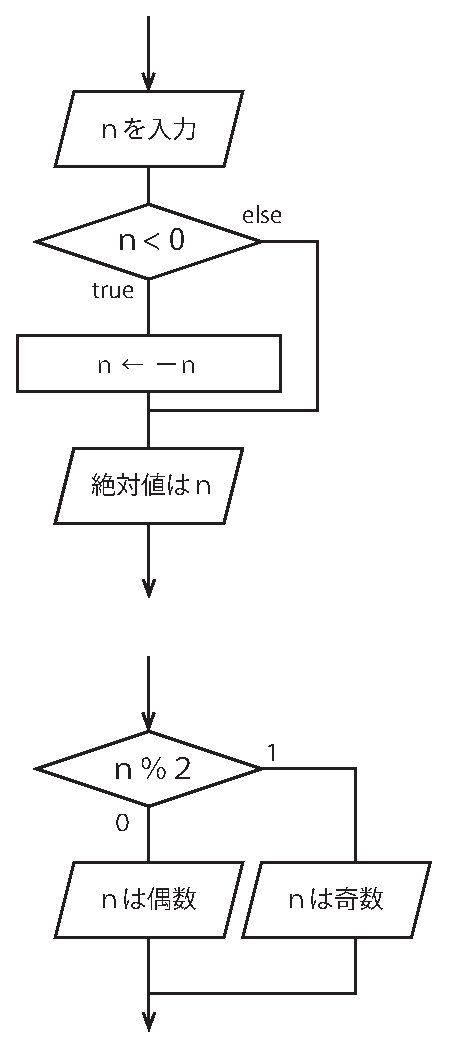
\includegraphics[scale=0.5]{figures/eps/odd-even.eps}
      \end{minipage}
    \end{tabular}
\end{figure}%

input('表示するメッセージ')関数を使って、標準出力(画面)にメッセージを表示させ、かつ標準入力(キーボード)から入力された値を、「文字列で」受け取ります。

受け取った文字列のままでは、かけ算をしたり割り算の余りを求めたりするような計算はできません。
演算を行うために、入力された文字列を int() によって整数に変換しています。

%何もしないでと言うときに、passというキーワードで指示をしている点にも注目しましょう。

\begin{table}[hbtp]
  \caption{比較演算子}
  \label{table:ope}
  \centering
  \begin{tabular}{l|l|l}
    \hline
    演算子  & \multicolumn{1}{c|}{意味}  &  使用例(Trueになる場合)\\
    \hline \hline
    ==  & 左辺と右辺が等しいならTrue & 10==10 \\
    !=  & 左辺と右辺が等しくないならTrue & 32!=10 \\
    \textgreater  & 左辺が右辺より大きいならTrue & 64\textgreater32 \\
    \textgreater=  & 左辺が右辺より大きいか又は等しいならTrue & 30\textgreater=20 \\
    \textless  & 左辺が右辺より小さいならTrue & 20\textless30 \\
    \textless=  & 左辺が右辺より小さいか又は等しいならTrue & 20\textless=20 \\
    \hline
  \end{tabular}
\end{table}

\textgreater= という演算子はありますが、=\textgreater という書き方はないので注意しましょう。

\textless= という演算子はありますが、=\textless という書き方はないので注意しましょう。

\subsection{elif}

if と else だけを使って記述すると、if文の入れ子(ネスト)が深くなってしまいます。

\begin{figure}[H]
  \centering
  \begin{tabular}{lr}
      \begin{minipage}{0.9\hsize}
      \centering
\lstinputlisting[caption=if-else,label=p02-2-1]{programs/python/p02-2-1.py}
      \end{minipage}
      \begin{minipage}{0.1\hsize}
      \flushright
%\includegraphics[scale=0.35]{if-else.eps}
      \end{minipage}
    \end{tabular}
\end{figure}%

\begin{center}
	\includegraphics[scale=0.45]{figures/eps/if-else.eps}
\end{center}

クォーテーション・マーク3個を連続させると、コメントの記述開始という意味になります。
コメントの記述終了も、クォーテーション・マークを3個を連続させて指示します。
#は1行ごとのコメントのために使い、クォーテーション・マーク3個を連続させるのは、複数行のコメントの場合に使います。

ここでは、乱数の発生させ方についても学習しましょう。
random()という関数は「0以上1未満の実数」による一様乱数を生成します。
一様乱数とは、「いかさまサイコロではないよ」という意味です。
乱数を使った模擬実験は、モンテカルロ・シミュレーションと呼ばれます。

elif を使うことによって、見やすいプログラムにすることができます。

\lstinputlisting[caption=elif,label=p02-2]{programs/python/p02-2.py}

Pythonでは、「$3/6$\textless= r \textless$4/6$」 という条件の書き方が許されています。
日本語の通常の言い方をすると「rは$3/6$と$4/6$の間の数である(また、$3/6$と等しいこともあり得る)」という意味ですね。
この書き方は自然な書き方の様に感じるかもしれませんが、この様な書き方ができるのはPythonだけです。

例えば
これと同じ条件をC言語やJavaで記述しようとすると、
「($3/6$ \textless= r) \&\& (r \textless $4/6$)」 という形で書かなければなりません。
つまり、「rは$3/6$以上であり、かつ$4/6$未満の数である」という書き方です。
(C言語やJavaで\&\&は、and「かつ」という意味でした)

Pythonにおける条件の書き方は簡易で分かりやすいのですが、
Python以外のプログラム言語、C言語やJavaではこの様な条件の記述はできない事を覚えておきましょう

なお、C言語やJavaには、switch-case文がありますが、Pythonにはありません。
if-elif-elseを使えば、switch-case文と同様の機能を実現できます。

また、elif というキーワードは、C言語やJavaでは、else if と書かれる部分に対応しています。

randomのいろいろ

\lstinputlisting[caption=random,label=p02-3]{programs/python/p02-3.py}

\newpage

\section{繰り返し}

\subsection{for文による繰り返し}

%\begin{lstlisting}[basicstyle=\ttfamily\footnotesize,frame=single]
\begin{lstlisting}
# Q1 文字列 '繰り返し' を5回印刷するには
print('繰り返し')
print('繰り返し')
print('繰り返し')
print('繰り返し')
print('繰り返し')
print('繰り返し終わり')

# A1 次のように for文 と range()関数を使って
for n in range(5):
    print('繰り返し')
print('繰り返し終わり')
\end{lstlisting}

range()関数の引数で、反復回数を指定していることを確認しましょう。

%\begin{lstlisting}[basicstyle=\ttfamily\footnotesize,frame=single]
\begin{lstlisting}
# Q2 文字列 '繰り返し' と '反復' の2行を 5回印刷するには
print('繰り返し')
print('反復')
print('繰り返し')
print('反復')
print('繰り返し')
print('反復')
print('繰り返し')
print('反復')
print('繰り返し')
print('反復')
print('繰り返し終わり')

# A2 次のように for文 と range()関数を使って
for n in range(5):
    print('繰り返し')
    print('反復')
print('繰り返し終わり')
\end{lstlisting}

for文の右端のコロン(:)の次の行から、反復する処理の範囲をインデントしています。

%\begin{lstlisting}[basicstyle=\ttfamily\footnotesize,frame=single]
\begin{lstlisting}
# Q3 文字列 '繰り返し' を5回印刷するとともに、繰り返し回数も一緒に印刷するなら
print('0 繰り返し')
print('1 繰り返し')
print('2 繰り返し')
print('3 繰り返し')
print('4 繰り返し')
print('繰り返し終わり')

# A3 次のように for文 と range()関数を使って
for n in range(5):
    print(n, '繰り返し')
print('繰り返し終わり')
\end{lstlisting}

for n ... において、関数range(5)によって、nには 0 から1,2,3,4 までの5個が、順に取り出されているのが分かります

%range()関数の引数が1つの場合、2つの場合、3つの場合のそれぞれの引数の意味を確認しましょう。

%また、どの場合でも反復を終了する時の値は、指定した値それ自身は含まれない点に、特に注意します。

\subsubsection{合計の計算}

次の計算をする処理をプログラムしてみましょう。
$n=10$の時、この計算結果は55になります。

\[
sum = \sum_{i=1}^{n}i = 1 + 2 + \cdots + (n-1) + n
\]

\begin{figure}[H]
  \centering
  \begin{tabular}{cc}
      \begin{minipage}{0.40\hsize}
      \centering
\lstinputlisting[caption=sum,label=p03-0]{programs/python/p03-0.py}
      \end{minipage}
      \begin{minipage}{0.4\hsize}
      \centering
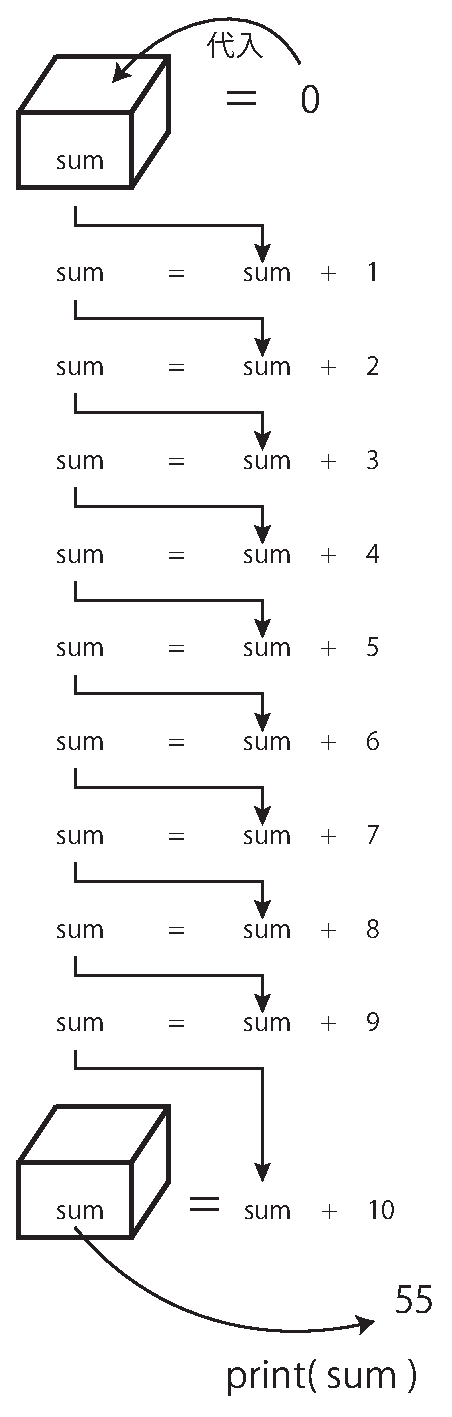
\includegraphics[scale=0.45]{figures/eps/sum.eps}
      \end{minipage}
    \end{tabular}
\end{figure}%

%\newpage

for文による繰り返し処理です。for文の右端にはコロン(:)を置き、
その次の行からインデントしたコードブロックを構成しなければなりません。

range()関数の使い方について、「要注意!」の部分をもう一度しっかり確認しましょう。

\lstinputlisting[caption=合計,label=p03-1]{programs/python/p03-1.py}

【演習問題】次の計算を、for文とrange()関数で記述しなさい

[1]$sum1 = 0 + (-1) + (-2) + \cdots + (-9) + (-10)$

[2]$sum2 = -10 + (-9) + \cdots + (-2) + (-1) + 0$

[3]$sum3 = -10 + (-8) + (-6) + (-4) + (-2) + 0$

[4]$factorial = 8 \times 7 \times \cdots \times 2 \times 1$

\subsubsection{階乗の計算}

合計sumと同様な繰り返し処理で、
階乗を計算するプログラムを書いてみます。

\[
fact = n! = n * ( n-1 ) * ( n-2 ) * \cdots * 3 * 2 * 1
\]

\lstinputlisting[caption=階乗,label=p03-2]{programs/python/p03-2.py}

\subsection{while文による繰り返し}

whileに続けて指定している条件が成り立っている間、インデントされたブロックが繰り返されます

\subsubsection{フィボナッチ数列}

最初の数は0、次の数は1と決めておいて、
3番目から後に続く数はすべて、直前の2つの数を加えた値になっているような数列を、フィボナッチ数列といいます

\begin{eqnarray*}
F_0 &=& 0\\
F_1 &=& 1\\
F_{k} &=& F_{k-1} + F_{k-2} \qquad (where \ k \geq 2)
\end{eqnarray*}

\lstinputlisting[caption=while,label=p03-2-1]{programs/python/p03-2-1.py}

\newpage

\subsubsection{breakとcontinue}

while True: によって、無限ループする処理をインデントしたブロックに作ることがあります

無限ループは、どこかでその繰り返しを終える条件を書く必要があります

\lstinputlisting[caption=breakとcontinue,label=p03-2-2]{programs/python/p03-2-2.py}

1から10までの整数の足し算をするという処理なので、nが10を超えたら繰り返しは終えて(breakして)いいのです。

また、nが1より小さい値の時はsumの計算をする必要がありませんから、次の値の繰り返しにすぐに入ります。

breakに遭遇すると、(その時の一番内側の)繰り返しを打ち切ります。

continueに当たると、その回だけはcontinue文以下は実行されずに、その次のループ処理に入ります。

\chapter{関数}

\section{関数、引数、戻り値}

プログラミングでは、

①入力があって、②その入力を元に何らかの処理をして、③その処理の結果を返す出力がある

という、3つを備えているものを関数と言っています

\begin{figure}[H]
  \centering
  \begin{tabular}{cc}
      \begin{minipage}{0.10\hsize}
      \centering
%\lstinputlisting[caption=sum,label=p03-0]{p03-0.py}
      \end{minipage}
      \begin{minipage}{0.9\hsize}
      \centering
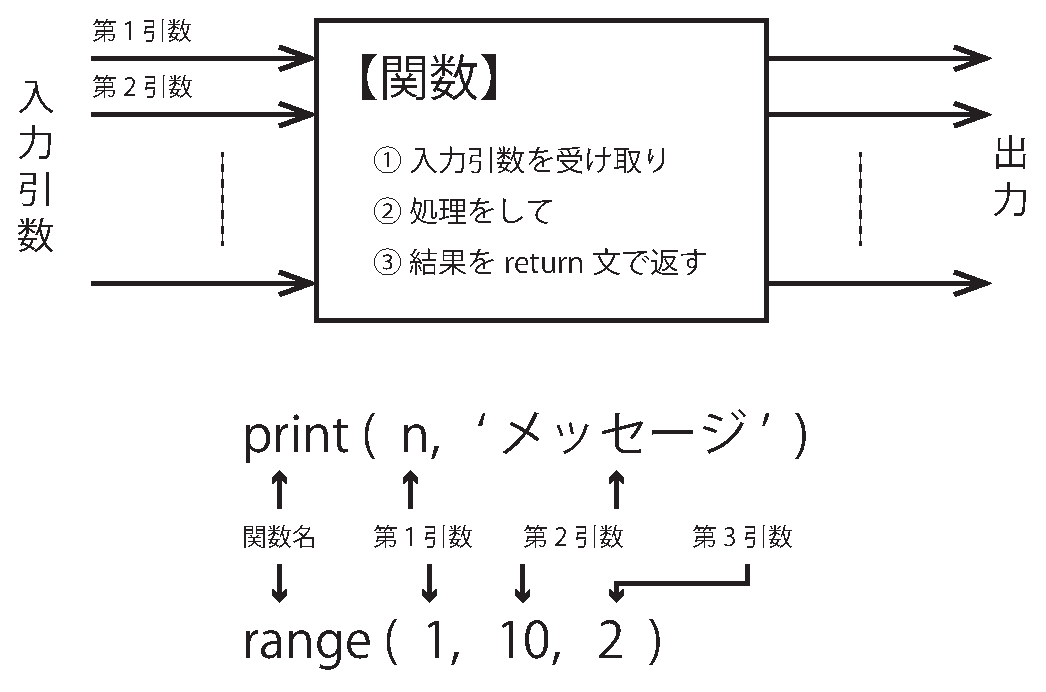
\includegraphics[scale=0.5]{figures/eps/func.eps}
      \end{minipage}
    \end{tabular}
\end{figure}%

これまで、print()関数やrange()関数を使ってきました

print()関数やrange()関数の、括弧内に指定している情報がそれぞれの関数に渡され、
それが関数では入力引数として受け取られて、それぞれの関数での処理が行われます

\subsubsection{戻り値のある関数}

\lstinputlisting[caption=関数定義,label=p03-1-3]{programs/python/p03-1-3.py}

関数定義の引数に書いている変数xは、
関数が入力引数として受け取る「仮の変数」として使います

この「仮の変数」を使って、関数内での処理を記述していきます

\subsubsection{戻り値のない関数}

%\begin{lstlisting}[basicstyle=\ttfamily\footnotesize,frame=single]
\begin{lstlisting}
# 絶対値を求める処理の関数定義です
def my_abs( x ):
    if x < 0:
        return -x
    return x

# 先ほどと同じ結果になります
a = my_abs( 5 )
b = my_abs( -10 )
print( 'a=', a )
print( 'b=', b )
c = a + my_abs( -10 ) + my_abs( 8 )
print( 'c=', c )

# 次の関数定義では、どうなるでしょう
def my_abs2( x ):
    if x < 0:
        return -x

# 引数xが負の数の場合に、-xを返すのは書かれていますから
d = my_abs2( -5 )
print( 'd=', d )

# 一方、引数xが正の数あるいはゼロの場合に、
# 関数の戻り値について書かれていません
e = my_abs2( 5 )
print( 'e=', e )

# None(ナン) という結果が返されています
# 次の様に、return文で何も指定しなかった場合もNoneが返されます
def my_abs3( x ):
    if x < 0:
        return -x
    return
#
print( my_abs3( -5 ) )
print( my_abs3(  5 ) )

# ちなみに、print()関数の戻り値もNoneになります
f = print( '戻り値を確認しよう' )
print( 'f=', f )
\end{lstlisting}

\subsection{再帰呼び出し}

フィボナッチ数列や階乗を求める関数は、再帰呼び出しを使って関数定義することができます。

\begin{figure}[htpb]
  \centering
  \begin{tabular}{c}
      \begin{minipage}{0.45\hsize}
      \begin{center}
\begin{lstlisting}[caption=,label=prog7]
def fib(n):
    '''
    n > 0 の整数を前提に、
    n 番目のフィボナッチ数を返す
    '''
    if n < 2:
        return n
    else:
        return fib(n-1) + fib(n-2)

n = 5
for i in range(n+1):
    print('fib of', i, '=', fib(i))
\end{lstlisting}
\end{center}
      \end{minipage}

\begin{minipage}{0.05\hsize}
  \begin{tabular}{c}

  \end{tabular}
\end{minipage}

      \begin{minipage}{0.40\hsize}
\begin{center}
\begin{lstlisting}[caption=,label=prog8]
def factorial(n):
    '''
    n > 0 の整数を前提に
    n! を返す
    '''
    if n <= 1:
        return 1
    else:
        return n * factorial(n-1)

n = 5
for i in range(n+1):
    print(i, '! = ', factorial(i))
\end{lstlisting}
\end{center}
      \end{minipage}
    \end{tabular}
\end{figure}%

\subsection{lambda関数}

匿名の(関数名を付けない)関数を定義することができます

\begin{lstlisting}[caption=,label=prog18]
c = (lambda a, b: 2*a + 3*b)(1.0, 4.0)
print(c)
data1 = [1, 2, 3, 4, 5]
data2 = [10, 9, 8, 7, 6]
result = list( map( lambda a, b: 2*a + 3*b, data1, data2 ) )
print(result)
\end{lstlisting}%

\section{順序引数、キーワード引数とデフォルト引数}

関数呼び出し時に「引数を渡した位置(順番)によって、どのパラメーターがその値を受け取るかが決定される」ような引数の渡し方を「位置引数」(positional argument)と呼ぶ。

関数呼び出し時に「実引数をどのパラメーターに渡すべきか」を「パラメーター名=実引数の値」のようにして指定する引数の渡し方を「キーワード引数」(keyword argument)と呼ぶ。

キーワード引数では、引数で受け取る値のデフォルト値を予め指定しておくことができる。その引数が指定されなかった場合に使われる。

位置引数とキーワード引数が混在する場合は、位置引数が先に書かれなければならない。

\begin{figure}[htpb]
  \centering
  \begin{tabular}{ll}
      \begin{minipage}{0.9\hsize}
      \centering
\begin{lstlisting}[caption=,label=prog7]
def funcArgs(arg1, arg2, arg3='three'):
    return f'arg1={arg1},arg2={arg2},arg3={arg3}'

print( funcArgs(1, 2, 3) )  # 位置引数
print( funcArgs( 'one', arg2='two') ) # 引数タイプの混在とデフォルト引数
print( funcArgs( 'one', arg3='four', arg2='two') )  # 混在では、位置引数が先
\end{lstlisting}%
      \end{minipage}
      \begin{minipage}{0.10\hsize}
      \centering
%\begin{lstlisting}[caption=,label=prog8]

%\end{lstlisting}
      \end{minipage}
    \end{tabular}
\end{figure}%

\section{変数のスコープ}

\begin{figure}[htpb]
  \centering
  \begin{tabular}{c}
      \begin{minipage}[t]{0.40\hsize}
      \centering
\begin{lstlisting}[caption=,label=prog7]
a = 10
def func1():
    a = 100
    print( 'a は local:', a )
def func2():
    global a
    a = 100
    print( 'a は global:', a )

func1()
print( a )
func2()
print( a )
\end{lstlisting}%
      \end{minipage}

      \begin{minipage}{0.05\hsize}
        \begin{tabular}{c}

        \end{tabular}
      \end{minipage}

      \begin{minipage}[t]{0.40\hsize}
      \centering
\begin{lstlisting}[caption=,label=prog8]
a = 10
print('a は global')
for i in range(10):
    print( a*i, end=' ' )

print('a は local')
for i in range(10):
    a = 2
    print( a*i, end=" " )
\end{lstlisting}
      \end{minipage}
    \end{tabular}
\end{figure}%

\lstinputlisting[caption=西暦と和暦を変換する関数を作ってみましょう,label=p03-1-2]{programs/python/p03-1-2.py}

\chapter{データ構造}

\section{文字列データの操作}

\begin{figure}[H]
  \centering
  \begin{tabular}{lr}
      \begin{minipage}{0.5\hsize}
      \centering
\lstinputlisting[caption=文字列,label=p01-1-1]{programs/python/p01-1-1.py}
      \end{minipage}
      \begin{minipage}{0.45\hsize}
      \flushright
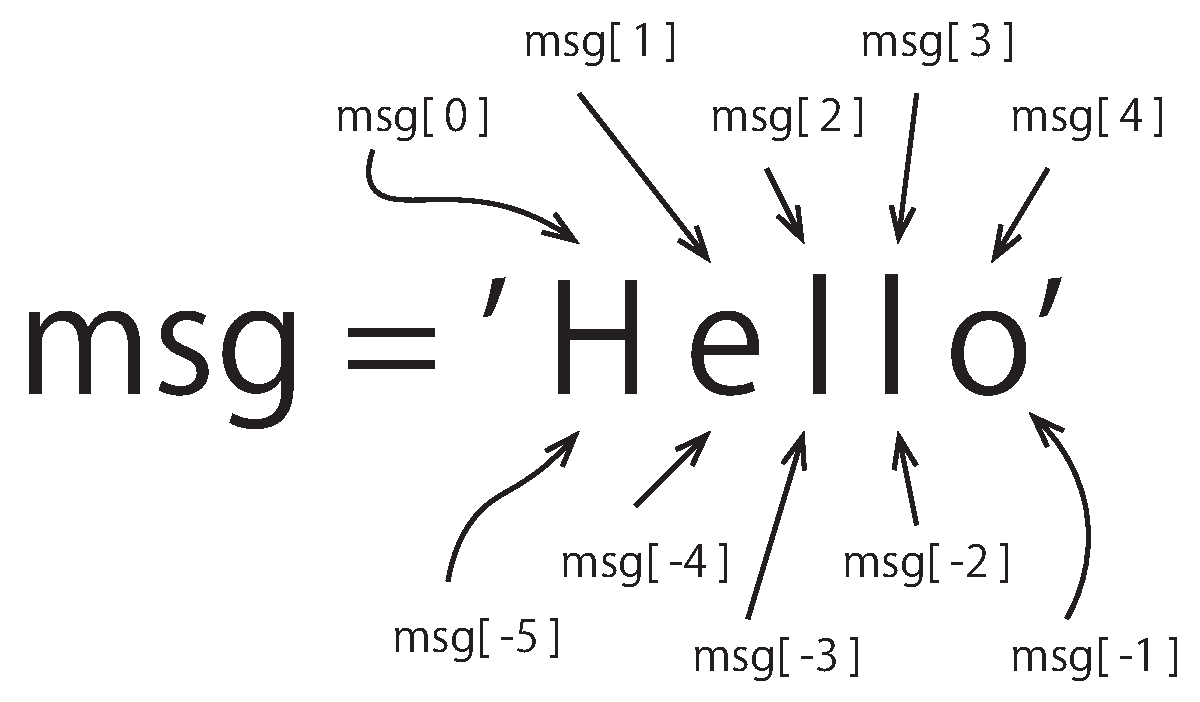
\includegraphics[scale=0.33]{figures/eps/fig2.eps}
      \end{minipage}
    \end{tabular}
\end{figure}%

文字列に対する色々な操作を示します

大文字、小文字の変換、及び文字列の置換は、何れも元の文字列に変更を加えているのではなく、
変換した後の新しい文字列オブジェクトを生成して、それを返してくれる関数になっています

\lstinputlisting[caption=文字列の操作いろいろ,label=p01-4-1]{programs/python/p01-4-1.py}

\section{リスト、タプル、辞書、集合(セット)}

\subsection{リスト}

リストとよばれるデータ構造に対する操作は、Pythonにおいて多用されます

リストは、複数の要素をカンマで区切って記述します。配列ともよばれます

例えばlistという名前の変数を、[5, 4, 3, 2]の様に、4つの要素がこの順番に入っているリスト(配列)とします

listの「0番目」の要素は、5です

listの「1番目」の要素は、4です

listの「2番目」の要素は、3です

listの「3番目」の要素は、2です

「0番目」とか「1番目」と言うときの数値のことを、リスト(配列)のインデックスと呼んでいます

リストの長さは、len()関数によって得られます(文字列の長さもlen()関数で得られましたね)

入れ子にすると、2次元配列を表せます

appendやinsert、popなどのメソッドを使うことによって、リストの内容を変更できます(このことをミュータブルという)

\begin{lstlisting}[caption=,label=prog6]
data = [3, 5, 2, 4, 3, 1]
print( data )

# リストの中で、一致する要素をカウントします
m = data.count( 3 )
print( m )

# リストの要素数(長さ)は
n = len( data )
print( n )

# index で要素を直接指定できます
print( data[0] )
print( data[n-1] )
print( data[-1] )

# index はコロン(:)で区切って、範囲を指定できます
print( data[1:3] )

# リストの最後に要素を追加
data.append( 8 )
print( data )
# リストの指定箇所に要素を追加
data.insert( 0, 8 )
print( data )
# リストの指定箇所の要素を取り出して削除
v = data.pop( 0 )
print( v )
print( data )
# del を使って、index で指定した要素を削除できます
del data[0]
print( data )
# index を指定しないと,リストそのものを削除してしまいます
del data
# print( data ) # dataが削除された後では,これはErrorになります

# 2次元配列
data2 = [[3, 5, 2], [4, 6, 1]]
print( data2[0] )
print( data2[0][1] )
print( data2[1] )

# アスタリスクの使い方に注目!
gdata = [ [0.0]*6 ]*5
print( gdata[0] )
print( gdata[2][4] )
\end{lstlisting}

\subsubsection{リストのコピー}

浅いコピーと深いコピーの違いを意識しておく必要があります。

\begin{figure}[htpb]
  \centering
  \begin{tabular}{c}
      \begin{minipage}{0.48\hsize}
      \centering
\begin{lstlisting}[caption=,label=prog7]
x = [1, 2, 3]
# これは、「浅いコピー」
y = x
# リストxの先頭番地が、yにコピーされた
# yもxも「同一のリスト要素」の先頭を保持
y[0] = 10
print( y )
print( x ) # x も更新されている
\end{lstlisting}%
      \end{minipage}

\begin{minipage}{0.04\hsize}
  \begin{tabular}{c}

  \end{tabular}
\end{minipage}

      \begin{minipage}{0.48\hsize}
      \centering
\begin{lstlisting}[caption=,label=prog8]
x = [1, 2, 3]
# これは、「深いコピー」
y = x.copy()
# リストxの値要素が、全てyにコピーされた
# yはxとは独立した配列要素を持っている
y[0] = 15 # y配列だけが更新された
print( y )
print( x ) # x は元のまま
\end{lstlisting}
      \end{minipage}
    \end{tabular}
\end{figure}%

【リストを使う例題】

\lstinputlisting[caption=breakとcontinue,label=p03-4]{programs/python/p03-4.py}

リストlistの中の要素の合計を求めるプログラムです

for文の中でenumerate()関数を使うことによって、
リストのインデックスと要素の両方を、それぞれ変数indexと、変数itemで受け取っています

\lstinputlisting[caption=while文,label=p03-5]{programs/python/p03-5.py}

%\newpage

\subsection{タプル}

タプル(tuple)型の変数は、リスト型と同様に複数の要素が順に並んでいる配列です

リストと違って、タプルで作成された要素は変更できません(読み出し専用の変数のことをイミュータブルという)

\begin{lstlisting}[caption=,label=prog9]
# 以下のt1,t2,t3は,いずれもtupleです
# リストは大括弧で囲みましたが、
# タプルは小括弧で囲みます
t1 = (1, 2, 3, 4, 3, 2, 1)
print( t1 )
print( type(t1) )
print( 't1の長さは、', len(t1) )
print( 't1の中で3の出現回数は,', t1.count(3) )

# 大括弧でインデックスの位置の要素を選ぶのは、タプルもリストも同じ方法です
print( 't1[2] + t1[4] = ', t1[2] + t1[4] )
# 小括弧ではタプルのインデックスを指定できません!
# print( 't1(2) + t1(4) = ', t1(2) + t1(4) ) # これは error になります

# 小括弧で囲まなくても、カンマで区切るだけでタプルを作れます
t2 = -1, -2, -3, -4
print( t2 )
print( type(t2) )
# 要素数1個のタプルの作り方(カンマ付きに注意!)
t3 = (1,)
print( t3 )
print( type(t3) )
# カンマを書かないと、小括弧で囲んでも単なる数値と見なされてしまいます
t4 = (1)
print( t4 )
print( type(t4) )
\end{lstlisting}%

\subsection{内包表記}

内包表記は、リストやタプルなどの順序型の変数の中の各要素に対して、簡易に演算を適用する方法のことです。
例えば、変数listを、次の様にして作ることがあります

\begin{verbatim}list = [ i for i in range(5, 1, -1) ]\end{verbatim}

変数list は、そもそも [i] という形のリストなのですが、
この変数 i を range(5, 1, -1) の範囲で変化させることを、
for i in range(5, 1, -1)の部分で行って、[5, 4, 3, 2]の形のリストを作っているのです

リストの中で処理を書いてしまうような方法をリスト内包表記といい、Pythonでは多用されます

\lstinputlisting[caption=リストによる繰り返し,label=p03-3]{programs/python/p03-3.py}

内包表記に、if文が書かれることもあります

\begin{lstlisting}[caption=,label=prog10]
# タプルを用意しておいて
t = (1, 2, 3, 4, 5)
# そのタプルのデータを元にしてリストを作っています
lst1 = [i for i in t]
print( lst1 )
# タプルtの中の要素を、forで順に取り出し、
# それが偶数の場合だけを、リストの要素にしています
lst2 = [i for i in t if i%2 == 0]
print( lst2 )
\end{lstlisting}%

\subsection{辞書型}

辞書(dict)型の変数は、キー(key)と値(value)がコロンで区切られたペアとして構成されます

辞書の各要素は順序づけられていないため、「何番目の要素」の様なアクセスはできません

各要素へは、キーを指定して、そのキーを持つ値にアクセスすることができます

\begin{lstlisting}[caption=,label=prog11]
# 一行が長くなるときは、バックスラッシュ(¥)を使って複数行に書くことができます
month = { '睦月': 1, '如月': 2, '弥生': 3, '卯月': 4,\
          '皐月': 5, '水無月': 6, '文月': 7, '葉月': 8,\
          '長月': 9, '神無月': 10, '霜月': 11, '師走': 12}
print( month )
dist = month['長月'] - month['卯月']
print( '長月'+'と'+'卯月'+'は、', dist, 'ヶ月はなれています\n' )

month['睦月'] = 'むつき'
month['如月'] = 'きさらぎ'
month['弥生'] = 'やよい'
month['卯月'] = 'うづき'
month['皐月'] = 'さつき'
month['水無月'] = 'みなづき'
month['文月'] = 'ふみづき'
month['葉月'] = 'はづき'
month['長月'] = 'ながつき'
month['神無月'] = 'かんなづき'
month['霜月'] = 'しもつき'
month['師走'] = 'しわす'
print( 'キーだけの一覧:', month.keys(), '\n'  )
print( '値だけ の一覧:', month.values(), '\n'  )
print( '辞書  の全体:', month, '\n' )
print( '如月 は、「' + month['如月'] + '」と読みます')
print( '皐月 は、「' + month['皐月'] + '」と読みます')
\end{lstlisting}%

\subsection{集合(セット)}

中括弧{}で要素を囲むとセット型オブジェクトを生成できる

重複する値がある場合は無視されて、一意な値のみが要素として残る

intやfloatのように異なる型でも値が等価であれば重複していると見なされる

異なる型を要素として持つこともできる。ただし、リスト型のような更新可能なオブジェクトは登録できない。タプルはOK

set型は順序をもたないので、生成時の順序は記憶されない

空の波括弧{}は辞書型dictと見なされるため、空のset型オブジェクト(空集合)を生成するには特別のコンストラクタset()を使う

\begin{lstlisting}[caption=,label=prog9]
# 中括弧{}で要素を囲むとセット型オブジェクトを生成できる
s = {1, 2, 2, 3, 1, 4}
print(s)
print(type(s))

# 集合の要素数は組み込み関数len()で取得できる
print( len(s) )

# set型は順序をもたないので、生成時の順序は記憶されない
s = {1.23, '百', (0, 1, 2), '百'}
print(s)

# intやfloatのように異なる型でも値が等価であれば重複していると見なされる
s = {100, 100.0}
print(s)

# リスト内包表記と同様に集合内包表記もある。
# リスト内包表記の角括弧[]を波括弧{}にするだけ
s = {i**2 for i in range(5)}
print(s)

# 集合に要素を追加するには、add()メソッドを使う
s = {0, 1, 2}
s.add(3)
print(s)

# 集合から要素を削除するには、discard(), remove(), pop(), clear()メソッドを使う
# discard()メソッドは引数に指定した要素を削除する。
# 集合に存在しない値を指定すると何もしない
s = {0, 1, 2}
s.discard(1)
print(s)

s = {0, 1, 2}
s.discard(10)
print(s)

# remove()メソッドも引数に指定した要素を削除するが、
# 集合に存在しない値を指定するとエラーKeyErrorになる
s.remove(1)
print(s)

s = {0, 1, 2}
s.remove(10)
# KeyError: 10

# pop()メソッドは集合から要素を削除し、その値を返す
# どの値を削除するかは選択できない。空集合だとエラーKeyErrorになる
s = {2, 1, 0}
v = s.pop()
print(s)
print(v)

s = {2, 1, 0}
print(s.pop())
print(s.pop())
print(s.pop())
print(s.pop())
# KeyError: 'pop from an empty set'

# clear()メソッドはすべての要素を削除し、空集合とする
s = {0, 1, 2}
s.clear()
print(s)
\end{lstlisting}%

和集合や積集合など、集合の演算に関するメソッドが用意されています。

\begin{lstlisting}[caption=,label=prog9]
# set型のオブジェクトはコンストラクタset()でも生成できる
# 引数としてリストやタプルのようなイテラブルオブジェクトを指定すると、
# 重複する要素が除外されて一意な値のみが要素となるsetオブジェクトが生成される
l = [1, 2, 2, 3, 1, 4]
print(l)
print(type(l))
s_l = set(l)
print(s_l)
print(type(s_l))

# イミュータブルなfrozenset型はコンストラクタfrozenset()で生成する
fs_l = frozenset(l)

print(fs_l)
print(type(fs_l))

# 引数を省略すると、空のset型オブジェクト(空集合)が生成される
s = set()
print(s)
print(type(s))

# set()を利用してリストやタプルから重複した要素を取り除くことができるが、
# 元のリストの順序は保持されない
# set型をリストやタプルに変換するにはlist(), tuple()を使う
l = [2, 2, 3, 1, 3, 4]
l_unique = list(set(l))
print(l_unique)

# 順序を保持したまま重複した要素を削除する場合や、
# 重複した要素のみを抽出したりする場合
# 二次元配列(リストのリスト)の重複要素を処理したい場合などについては別途

# 和集合(合併、ユニオン)は|演算子またはunion()メソッドで取得できる
s2 = {1, 2, 3}
s3 = {2, 3, 4}
s_union = s1 | s2
print(s_union)
s_union = s1.union(s2)
print(s_union)

# メソッドには複数の引数を指定することができる。また集合set型だけでなく、
# set()でset型に変換できるリストやタプルなども引数に指定できる。
# 以降の演算子、メソッドも同様
print(s_union)
s_union = s1.union(s2, [5, 6, 5, 7, 5])
print(s_union)

# 積集合(共通部分、交差、インターセクション)は&演算子
# またはintersection()メソッドで取得できる
print(s_intersection)

s_intersection = s1.intersection(s2)
print(s_intersection)

s_intersection = s1.intersection(s2, s3)
print(s_intersection)

# 差集合は-演算子またはdifference()メソッドで取得できる
s_difference = s1 - s2
print(s_difference)

s_difference = s1.difference(s2)
print(s_difference)

s_difference = s1.difference(s2, s3)
print(s_difference)

# 対称差集合(どちらか一方にだけ含まれる要素の集合)は^演算子
# またはsymmetric_difference()で取得できる
# 論理演算における排他的論理和(XOR)に相当
s_symmetric_difference = s1 ^ s2
print(s_symmetric_difference)

s_symmetric_difference = s1.symmetric_difference(s2)
print(s_symmetric_difference)

# ある集合が別の集合の部分集合かを判定するには、<=演算子
# またはissubset()メソッドを使う
s1 = {0, 1}
s2 = {0, 1, 2, 3}

print(s1 <= s2)
print(s1.issubset(s2))

# <=演算子もissubset()メソッドも、等価な集合に対してTrueを返す
# 真部分集合であるかを判定するには、等価な集合に対してFalseを返す<演算子を使う
print(s1 <= s1)
print(s1.issubset(s1))
print(s1 < s1)

# ある集合が別の集合の上位集合かを判定するには、>=演算子またはissuperset()を使う
s1 = {0, 1}
s2 = {0, 1, 2, 3}
print(s2 >= s1)
print(s2.issuperset(s1))

# >=演算子もissuperset()メソッドも、等価な集合に対してTrueを返す
# 真上位集合であるかを判定するには、等価な集合に対してFalseを返す>演算子を使う
print(s1 >= s1)
print(s1.issuperset(s1))
print(s1 > s1)

# 二つの集合が互いに素かを判定するには、isdisjoint()メソッドを使う
s1 = {0, 1}
s2 = {1, 2}
s3 = {2, 3}
print(s1.isdisjoint(s2))
print(s1.isdisjoint(s3))
\end{lstlisting}%

\chapter{実践演習}

\section{数独}

再帰呼び出しについて学習する一つの例として、数独を解くプログラムを考えます

最初に、boardリストに盤面を定義し、盤面の印刷を行う関数print\_board()を定義します

まずは、print\_board()をそのまま呼び出して動作を確認してみましょう

\begin{lstlisting}[caption=board,label=sudoku01]
board = [[5,3,0,0,7,0,0,0,0],\
         [6,0,0,1,9,5,0,0,0],\
         [0,9,8,0,0,0,0,6,0],\
         [8,0,0,0,6,0,0,0,3],\
         [4,0,0,8,0,3,0,0,1],\
         [7,0,0,0,2,0,0,0,6],\
         [0,6,0,0,0,0,2,8,0],\
         [0,0,0,4,1,9,0,0,5],\
         [0,0,0,0,8,0,0,7,9]]

def print_board():
    global board
    for y in range(9):
        for x in range(9):
            print(' ',end='')
            if x in [2,5]:
                print(board[y][x], end=' |')
            else:
                print(board[y][x], end=' ')
        if y in [2,5]:
            print('\n---------|---------|--------')
        else:
            print()

# 動作確認
print_board()
\end{lstlisting}

\begin{verbatim}
  5  3  0 | 0  7  0 | 0  0  0
  6  0  0 | 1  9  5 | 0  0  0
  0  9  8 | 0  0  0 | 0  6  0
 ---------|---------|--------
  8  0  0 | 0  6  0 | 0  0  3
  4  0  0 | 8  0  3 | 0  0  1
  7  0  0 | 0  2  0 | 0  0  6
 ---------|---------|--------
  0  6  0 | 0  0  0 | 2  8  0
  0  0  0 | 4  1  9 | 0  0  5
  0  0  0 | 0  8  0 | 0  7  9
\end{verbatim}

次に、引数yとxで指定されたスロットに、
第三引数で受け取ったnを置く事ができるか否かを判定する関数possible()を定義します

(1) 縦一列の中に、nと同じ数字があったら置けませんので、Falseを返します

(2) 横一行の中に、nと同じ数字があったら置けませんので、Falseを返します

(3) 3$\times$3の枠の中に、nと同じ数字があったら置けませんので、Falseを返します

上記(1)、(2)、(3)の何れでもないなら、Trueを返します

5行5列目(boardリストの0行目や0列目から数え始めるので、引数はx=y=4)の空きスロットに値を指定して、possible()の動作を確認しましょう

\begin{lstlisting}[caption=possible,label=sudoku02]
def possible(y,x,n):
    global board
    for i in range(0,9):
        if board[y][i] == n:
            return False
    for i in range(0,9):
        if board[i][x] == n:
            return False
    x0 = (x//3)*3
    y0 = (y//3)*3
    for i in range(0,3):
        for j in range(0,3):
            if board[y0+i][x0+j] == n:
                return False
    return True

# 動作確認
print( possible(4,4,4) )
print( possible(4,4,5) )
\end{lstlisting}

最後に、問題を解く関数solve()を定義します

y行x列目のスロットに着目して、そこが0ならば空きスロットですから、
そのスロットに、1から10までの数字を順に指定して、possible()を呼びだしてはチェックしていきます

もし、possible()関数がTrueを返したら、それは一つの候補ですので、
引き続きsolve()を繰り返して空きスロットを埋めていきます

solve()がreturnでNoneを返したときは、選ばれた候補は使えなかったという事ですので、
盤面のスロットを空(0)に戻しています

全ての空欄が埋まったなら、print\_board()を呼んで結果(答え)を印刷しています

\begin{lstlisting}[caption=solve,label=sudoku03]
def solve():
    global board
    for y in range(9):
        for x in range(9):
            if board[y][x] == 0:
                for n in range(1,10):
                    if possible(y,x,n):
                        board[y][x] = n
                        solve()
                        board[y][x] = 0
                return
    print_board()

# 動作確認
solve()
\end{lstlisting}

solve()関数の中から、自分自身であるsolve()関数を呼び出しています。再帰呼び出しです。
再帰呼び出しを使うことによって、プログラムを短く記述できています

実行結果

\begin{verbatim}
  5  3  4 | 6  7  8 | 9  1  2
  6  7  2 | 1  9  5 | 3  4  8
  1  9  8 | 3  4  2 | 5  6  7
 ---------|---------|--------
  8  5  9 | 7  6  1 | 4  2  3
  4  2  6 | 8  5  3 | 7  9  1
  7  1  3 | 9  2  4 | 8  5  6
 ---------|---------|--------
  9  6  1 | 5  3  7 | 2  8  4
  2  8  7 | 4  1  9 | 6  3  5
  3  4  5 | 2  8  6 | 1  7  9
\end{verbatim}

プログラムで解けてしまうとなると、しかも「こんなに短いプログラムで」解いたとなると、
数独そのものはつまらないものになりますね。
また「1から9まで総当たりで試しながら」=「コンピュータが力ずくで」なので、芸がないという気がします

このゲームは、まずは鉛筆と消しゴムを使って、自分で解いてみることが楽しむための重要なポイントのようです

【演習】

\section{三目並べ(Tic-Tac-Toe)}

プログラムを実行すると盤面が表示され、×の石を置く場所を指定するよう促されます

既に石の置かれているスロット番号は指定できませんし、スロット番号として 0 〜 8 の数値を指定しなければなりません

キーボードから番号を入力すると、その番号のスロットに×の石が置かれた盤面が表示され、
次の手番のコンピュータは、乱数で決めた場所に○を置いてきます

手番を交互に変えながらゲームは進み、縦、横、斜めの何れかに、先に一列に自分の石を並べた方が勝ちとなります

\begin{spacing}{0.74}
  \begin{verbatim}
    スタート! [Tic Tac Toe]
    /---|---|---\
    | 0 | 1 | 2 |
    |---|---|---|
    | 3 | 4 | 5 |
    |---|---|---|
    | 6 | 7 | 8 |
    \---|---|---/
    あなたの手番です。スロット番号は? : 4
    /---|---|---\
    | 0 | 1 | 2 |
    |---|---|---|
    | 3 | X | 5 |
    |---|---|---|
    | 6 | 7 | 8 |
    \---|---|---/
    /---|---|---\
    | 0 | 1 | O |
    |---|---|---|
    | 3 | X | 5 |
    |---|---|---|
    | 6 | 7 | 8 |
    \---|---|---/
    あなたの手番です。スロット番号は? :
        ・
        ・
        ・
  \end{verbatim}
\end{spacing}

三目並べの盤面boardをリストで用意し、それを画面に表示する関数print\_board()を定義します

空きスロットは0(スペース)、人が置いた石は1(X)、コンピュータが置いた石は2(O)を、boardに代入することにします

\begin{lstlisting}[caption=board,label=tictactoe01]
board = [0,0,0,\
         0,0,0,\
         0,0,0]

def print_board():
    global board
    bd = ['', '', '',\
          '', '', '',\
          '', '', '']
    for val in board:
        if val==0:
            bd[n] = ' '
        elif val==1:
            bd[n] = 'X'
        elif val==2:
            bd[n] = 'O'
        n += 1
    print( '/---|---|---\\')
    print( '| {} | {} | {} |'.format(bd[0], bd[1], bd[2]) )
    print( '|---|---|---|')
    print(f'| {bd[3]} | {bd[4]} | {bd[5]} |')
    print( '|---|---|---|')
    print(f'| {bd[6]} | {bd[7]} | {bd[8]} |')
    print( '\\---|---|---/')

# 動作確認
print_board()
\end{lstlisting}%

コンピュータは乱数でスロット番号を選び、そこが空きスロットなら2をboardに代入します

\begin{lstlisting}[caption=machine_put,label=tictactoe02]
from random import randint
def machine_put():
    global board
    while True:
        n = randint(0:8)
        if board[n]==0:
            board[n] = 2
            break

# 動作確認
machine_put()
board_print()
\end{lstlisting}%

人の手番では入力を促すメッセージを表示し、(整数の入力を期待していますが)
キーボードから入力された整数が空きのスロット番号として有効なら、
そこに1を代入します

\begin{lstlisting}[caption=human_put,label=tictactoe03]
def human_put():
    global board
    while True:
        instr = input("あなたの手番です。スロット番号は? : ")
        n = int( instr )
        if 0<=n<9 and board[n] == 0:
            board[n] = 1
            break

# 動作確認
human_put()
print_board()
\end{lstlisting}%

縦、横、斜めに一致したなら、勝敗がついたという意味でTrueを返し、
そうでなければ、ゲーム継続ですのでFalseを返します

\begin{lstlisting}[caption=judge,label=tictactoe04]
def judge():
    global board
    if  board[0]==board[1]==board[2] or\
        board[3]==board[4]==board[5] or\
        board[6]==board[7]==board[8] or\
        board[0]==board[3]==board[6] or\
        board[1]==board[4]==board[7] or\
        board[2]==board[5]==board[8] or\
        board[0]==board[4]==board[8] or\
        board[2]==board[4]==board[6]:
        return True
    return False
\end{lstlisting}%

ゲーム全体の流れは、start\_game()関数に定義します

\begin{lstlisting}[caption=game,label=tictactoe05]
def start_game():
    print("スタート! [Tic Tac Toe]")
    machine_turn = False
    while True:                         # 以下をゲームオーバーまで繰り返す
        board_print()                   # 盤面を表示して
        if machine_turn:                # machineの手番なら
            machine_put()
        else:                           # humanの手番なら
            human_put()
        if judge():                     # 勝敗の判定
            break
        machine_turn = not machine_turn # 手番を交代する

# 動作確認
start_game()
\end{lstlisting}%



【演習】

\section{ライフゲーム}

\url{http://vigne-cla.com/17-1/}

フィールドは正方形のマス目で、各マスの状態が変化するためのルールは次の2つだけです。

現在の状態	隣接する8セルの条件	次の状態
生存(1)	生存セルが0~1または4~8個	死(0)
死(0)	生存セルが3個	生存(1)
これに当てはまらない場合は現状維持となります。

別の表現として、生きるための条件に着目して書くとこうなります。

次のステップでの生存条件
生存セル	隣接する8セルのうち生存セルが2、3個
死セル	隣接する8セルのうち生存セルが3個


\begin{lstlisting}[caption=life00,label=life00]
import numpy as np
import numpy.random as nr
import matplotlib.pyplot as plt

#============================
#初期状態の設定(グライダー)
#============================

#高さ、幅
h, w = 10, 10

#任意の状態を用意
state = np.array([[0,0,1],
                  [1,0,1],
                  [0,1,1]])

#フィールドのどこに置くか(左上点を指定)
p = (0, 0)

#終了ステップ数
max_step = 35

#============================
#メイン処理
#============================

#フィールドの生成
f = np.zeros((h, w), dtype=bool)

#任意の状態を置く
f[p[0]:p[0]+len(state), p[1]:p[1]+len(state[0])] = state

#初期状態の表示
#plt.figure(figsize=(10, 10))
plt.imshow(f, cmap='inferno')
#plt.savefig('save/{}.png'.format(0), bbox_inches='tight', pad_inches=0)
plt.show(), print()

#状態の更新
for i in range(1, max_step + 1):

    #周囲の生存マス数を記録するための配列
    mask = np.zeros((h, w))

    #周囲の生存マスを足し込む
    mask[1:, :] += f[:-1, :] #上
    mask[:-1, :] += f[1:, :] #下
    mask[:, 1:] += f[:, :-1] #左
    mask[:, :-1] += f[:, 1:] #右
    mask[1:, 1:] += f[:-1, :-1] #左上
    mask[1:, :-1] += f[:-1, 1:] #右上
    mask[:-1, 1:] += f[1:, :-1] #左下
    mask[:-1, :-1] += f[1:, 1:] #右下

    #未来のフィールド(すべて死状態)
    future = np.zeros((h, w), dtype=bool)

    #生きているマスが生きる条件(=生存)
    future[mask*f==2] = 1
    future[mask*f==3] = 1
    #死んでいるマスが生きる条件(=誕生)
    future[mask*~f==3] = 1

    #フィールドの更新(浅いコピーに注意)
    f = future

    #表示
    #plt.figure(figsize=(10, 10))
    plt.imshow(f, cmap='inferno')
    #plt.savefig('save/{}.png'.format(i), bbox_inches='tight', pad_inches=0)
    plt.show(), print()
\end{lstlisting}%

\begin{lstlisting}[caption=life01,label=life01]
#============================
#初期状態の設定(銀河)
#============================

#高さ、幅
h, w = 15, 15

#任意の状態を用意
state = np.array([[1,1,0,1,1,1,1,1,1],
                  [1,1,0,1,1,1,1,1,1],
                  [1,1,0,0,0,0,0,0,0],
                  [1,1,0,0,0,0,0,1,1],
                  [1,1,0,0,0,0,0,1,1],
                  [1,1,0,0,0,0,0,1,1],
                  [0,0,0,0,0,0,0,1,1],
                  [1,1,1,1,1,1,0,1,1],
                  [1,1,1,1,1,1,0,1,1]])

#フィールドのどこに置くか(左上点を指定)
p = (3, 3)

#終了ステップ数
max_step = 15
\end{lstlisting}%

\begin{lstlisting}[caption=life02,label=life02]
#============================
#初期状態の設定(ダイハード)
#============================

#高さ、幅
h, w = 25, 25

#任意の状態を用意
state = np.array([[0,0,0,0,0,0,1,0],
                  [1,1,0,0,0,0,0,0],
                  [0,1,0,0,0,1,1,1]])

#フィールドのどこに置くか(左上点を指定)
p = (5, 9)

#終了ステップ数
max_step = 135
\end{lstlisting}%

\begin{lstlisting}[caption=life03,label=life03]
#============================
#初期状態の設定(十字スタート)
#============================

#高さ、幅
h, w = 401, 401

#任意の状態を用意
state = np.zeros((h, w))
state[200, :] = 1
state[:, 200] = 1

#フィールドのどこに置くか(左上点を指定)
p = (0, 0)

#終了ステップ数
max_step = 135
\end{lstlisting}%

\begin{comment}

\section{オセロ(リバーシ)}

オセロという名前は、シェイクスピアの戯曲「オセロ」がその由来だということです。
黒白の石がひっくり返りながら、形勢が次々と変わっていくというゲーム性が、
戯曲における、黒人の将軍オセロと白人の妻デスデモーナを中心に、
敵味方がめまぐるしく寝返るというストーリーを連想させるということから、
このゲームをオセロと名付けることにしたということです。

8 $\times$ 8サイズのゲームが一般的ですが、
6 $\times$ 6盤の縮小オセロでは必勝法が見つかっているようです

1993年にイギリスのJoel Feinsteinが、6 $\times$ 6盤の縮小オセロで、
先手が最善手を尽くしたとしても、後手が「20対16」で勝つ
(先手16対後手20で、後手の4目勝ち)となる事を示したということです

ここでは、
4 $\times$ 4「以上」の大きさの盤面に対応するオセロを作ります

以下のゲーム例では、×(BLACK)の手番ですが、○(WHITE)を裏返せないところに×を置こうとしたり、
×(BLACK)を置ける場所があるのにpassを宣言したりすると、再入力を促されています

○(WHITE)の手番では、乱数によってコンピュータが石を置くスロットを決めています

\begin{spacing}{0.74}
\begin{verbatim}
  WHITE:2, BLACK:2
    0 1 2 3 →x
  0 . . . .
  1 . X O .
  2 . O X .
  3 . . . .
  ↓
  y
  Your turn. [yx] or "pass": 23
  Your turn. [yx] or "pass": pass
  Your turn. [yx] or "pass": 13

  WHITE:1, BLACK:4
    0 1 2 3 →x
  0 . . . .
  1 . X X X
  2 . O X .
  3 . . . .
  ↓
  y
  WHITE:3, BLACK:3
    0 1 2 3 →x
  0 . . . .
  1 . X X X
  2 . O O O
  3 . . . .
  ↓
  y
  Your turn. [yx] or "pass": 33

  WHITE:1, BLACK:6
    0 1 2 3 →x
  0 . . . .
  1 . X X X
  2 . O X X
  3 . . . X
  ↓
  y
  WHITE:3, BLACK:5
    0 1 2 3 →x
  0 . O . .
  1 . O X X
  2 . O X X
  3 . . . X
  ↓
  y
  Your turn. [yx] or "pass": 00

  ( ・・ 途中略 ・・ )

  WHITE:5, BLACK:9
    0 1 2 3 →x
  0 X X X O
  1 O X X X
  2 O O X X
  3 O . . X
  ↓
  y
  Your turn. [yx] or "pass": 31

  WHITE:4, BLACK:11
    0 1 2 3 →x
  0 X X X O
  1 O X X X
  2 O X X X
  3 O X . X
  ↓
  y
  WHITE:7, BLACK:9
    0 1 2 3 →x
  0 X X X O
  1 O X X X
  2 O O X X
  3 O O O X
  ↓
  y

  Winner : BLACK
\end{verbatim}
\end{spacing}

\end{comment}
%\chapter{オブジェクト指向}

%別冊「Games with Python」参照

\begin{comment}
\section{スカッシュ・ゲーム}

\subsection{画面のクラス}

\begin{lstlisting}[caption=Class Screen,label=p2]
import pygame

class Screen:
    def __init__(self, width=600, height=600):
        self.WIDTH = width
        self.HEIGHT = height
        self.SIZE = (width, height)
        self.surface = pygame.display.set_mode( self.SIZE )

    def fill(self, color=(255, 255, 255)):
        self.surface.fill( color )

    def caption(self, str):
        pygame.display.set_caption( str )
\end{lstlisting}

\begin{lstlisting}[caption=main.py(1),label=p1]
import sys
import pygame
from pygame.locals import QUIT
from Screen import Screen

class Game():
    def __init__(self):
        pygame.init()
        self.WIDTH = 640
        self.HEIGHT = 480
        self.screen = Screen( self.WIDTH, self.HEIGHT )
        self.screen.caption( "Squash game" )
        self.clock = pygame.time.Clock()
        self.FPS = 30

    def fine(self):
        pygame.quit()
        sys.exit()

    def key_event(self):
        for event in pygame.event.get():
            if event.type == QUIT:
                self.fine()

    def start(self):
        game_over = False
        while not game_over:
            self.key_event()
            self.screen.fill()
            # ↓ ここからゲームを記述していく

            # ↑ ゲームの記述はここまで
            pygame.display.update()
            self.clock.tick(self.FPS)

if __name__ == '__main__':
    game = Game()
    game.start()
\end{lstlisting}

\subsection{ボールのクラス}

\begin{lstlisting}[caption=Class Ball,label=p3]
from math import sin, cos, radians
from random import randint
import pygame
from pygame.locals import Rect

class Ball( Rect ):
    def __init__(self, surface, color=(180, 180, 180),\
                        diameter=20, speed=10, start=(300,300)):
        self.surface = surface
        self.COLOR = color
        self.SPEED = speed
        ANGLE = 30
        self.dir = randint(ANGLE, 180 - ANGLE)
        self.left = start[0]
        self.top = start[1]
        self.width = diameter
        self.height = diameter

    def stop_ball(self):
        self.SPEED = 0

    def movex(self):
        self.centerx += int( cos(radians(self.dir)) * self.SPEED )

    def movey(self):
        self.centery += int( sin(radians(self.dir)) * self.SPEED )

    def movexy(self):
        self.movex()
        self.movey()

    def draw(self):
        pygame.draw.ellipse(self.surface, self.COLOR, self)
\end{lstlisting}

\begin{lstlisting}[caption=main.py(2),label=p1]
import sys
import pygame
from pygame.locals import QUIT
from Ball import Ball
from Screen import Screen

class Game():
    def __init__(self):
        pygame.init()
        self.WIDTH = 640
        self.HEIGHT = 480
        self.screen = Screen( self.WIDTH, self.HEIGHT)
        self.screen.caption("Squash game")
        self.clock = pygame.time.Clock()
        self.FPS = 30
        RED = (255,0,0)
        self.ball = Ball(self.screen.surface, color=RED)

    def fine(self):
        pygame.quit()
        sys.exit()

    def key_event(self):
        for event in pygame.event.get():
            if event.type == QUIT:
                self.fine()

    def boundary(self, ball):
        if not (0 <= ball.centerx <= self.WIDTH):
            ball.dir = 180 - ball.dir
        if not (0 <= ball.centery <= self.HEIGHT):
            ball.dir = -ball.dir

    def start(self):
        game_over = False
        while not game_over:
            self.key_event()
            self.screen.fill()
            self.ball.draw()
            self.boundary( self.ball )
            self.ball.movexy()
            pygame.display.update()
            self.clock.tick(self.FPS)

if __name__ == '__main__':
    game = Game()
    game.start()
\end{lstlisting}

\subsection{ラケットのクラス}

\begin{lstlisting}[caption=Class Racket,label=p4]
import pygame
from pygame.locals import Rect

class Racket(Rect):
    def __init__(self, surface, color=(20, 100, 150), left=300, top=300, width=80, height=10):
        self.surface = surface
        self.COLOR = color
        self.left = left
        self.top = top
        self.width = width
        self.height = height

    def movex(self, delx):
        self.centerx += delx

    def movey(self, dely):
        self.centery += dely

    def draw(self):
        pygame.draw.rect(self.surface, self.COLOR, self)
\end{lstlisting}

\begin{lstlisting}[caption=main.py(3),label=p1]
import sys
import pygame
from pygame.locals import QUIT, KEYDOWN, K_LEFT, K_RIGHT
from Ball import Ball
from Racket import Racket
from Screen import Screen

class Game():
    def __init__(self):
        pygame.init()
        self.WIDTH = 640
        self.HEIGHT = 480
        self.screen = Screen( self.WIDTH, self.HEIGHT)
        self.screen.caption("Squash game")
        self.clock = pygame.time.Clock()
        self.FPS = 30
        RED = (255,0,0)
        self.ball = Ball(self.screen.surface, color=RED)
        left = self.WIDTH//2
        top = self.HEIGHT - 50
        self.racket = Racket(self.screen.surface, left=left, top=top)
        pygame.key.set_repeat(10, 10)

    def fine(self):
        pygame.quit()
        sys.exit()

    def key_event(self):
        for event in pygame.event.get():
            if event.type == QUIT:
                self.fine()
            elif event.type == KEYDOWN:
                if event.key == K_LEFT and self.racket.left > 0:
                    self.racket.movex(-3)
                elif event.key == K_RIGHT and self.racket.right < self.WIDTH:
                    self.racket.movex(3)

    def hitted(self, racket, ball):
        if racket.colliderect( ball ):
            ball.dir = -(90 + (racket.centerx - ball.centerx) / racket.width * 100)

    def boundary(self, ball):
        if not (0 <= ball.centerx <= self.WIDTH):
            ball.dir = 180 - ball.dir
        if not (0 <= ball.centery <= self.HEIGHT):
            ball.dir = -ball.dir

    def start(self):
        game_over = False
        while not game_over:
            self.key_event()
            self.screen.fill()
            self.ball.draw()
            self.racket.draw()
            self.hitted( self.racket, self.ball )
            self.boundary( self.ball )
            self.ball.movexy()
            pygame.display.update()
            self.clock.tick(self.FPS)

if __name__ == '__main__':
    game = Game()
    game.start()
\end{lstlisting}

\subsection{メッセージ表示のクラス}

\begin{lstlisting}[caption=Class Message,label=p4]
import pygame

class Mess:
    def __init__(self, surface, size=80, color=(255,255,0)):
        self.surface = surface
        self.SIZE = size
        self.COLOR = color
        self.font = pygame.font.Font(None, size)
        self.MESSAGE = 'Hello'
        self.XPOS = self.YPOS = 0

    def display(self):
        text = self.font.render(self.MESSAGE, True, self.COLOR)
        textpos = text.get_rect()
        textpos.centerx = self.XPOS
        textpos.centery = self.YPOS
        self.surface.blit(text, textpos)

class Message( Mess ):
    def __init__(self, surface, message, xpos, ypos, size=80, color=(0,0,0)):
        super().__init__(surface, size, color)
        self.MESSAGE = message
        self.XPOS = xpos
        self.YPOS = ypos
\end{lstlisting}

\begin{lstlisting}[caption=main.py(4),label=p1]
import sys
import pygame
from pygame.locals import QUIT, KEYDOWN, K_LEFT, K_RIGHT
from random import randint
from Ball import Ball
from Message import Message
from Racket import Racket
from Screen import Screen

class Game():
    def __init__(self):
        pygame.init()
        self.WIDTH = 640
        self.HEIGHT = 480
        self.screen = Screen( self.WIDTH, self.HEIGHT)
        self.screen.caption("Squash game")
        self.clock = pygame.time.Clock()
        self.FPS = 30
        RED = (255,0,0)
        START = ( randint(0,self.WIDTH-1),0 )
        self.ball = Ball( self.screen.surface, color=RED, start=START )
        left = self.WIDTH//2
        top = self.HEIGHT - 50
        self.racket = Racket(self.screen.surface, left=left, top=top)
        xpos = left
        ypos = self.HEIGHT//2
        YELLOW = (255,255,0)
        self.msg_gover = Message( self.screen.surface, 'Game Over!!',\
                                  xpos, ypos, color=YELLOW )
        pygame.key.set_repeat(10, 10)

    def fine(self):
        pygame.quit()
        sys.exit()

    def key_event(self):
        for event in pygame.event.get():
            if event.type == QUIT:
                self.fine()
            elif event.type == KEYDOWN:
                if event.key == K_LEFT and self.racket.left > 0:
                    self.racket.movex(-3)
                elif event.key == K_RIGHT and self.racket.right < self.WIDTH:
                    self.racket.movex(3)

    def hitted(self, racket, ball):
        if racket.colliderect( ball ):
            ball.dir = -(90 + (racket.centerx - ball.centerx) / racket.width * 100)

    def boundary(self, ball):
        if not (0 <= ball.centerx <= self.WIDTH):
            ball.dir = 180 - ball.dir
        if ball.centery < 0:
            ball.dir = -ball.dir
        if self.HEIGHT < ball.centery:
            ball.stop_ball()
            self.msg_gover.display()

    def start(self):
        game_over = False
        while not game_over:
            self.key_event()
            self.screen.fill()
            self.ball.draw()
            self.racket.draw()
            self.hitted( self.racket, self.ball )
            self.boundary( self.ball )
            self.ball.movexy()
            pygame.display.update()
            self.clock.tick(self.FPS)

if __name__ == '__main__':
    game = Game()
    game.start()
\end{lstlisting}

\newpage

\section{ブロック崩しゲーム}

\subsection{ブロックのクラス}

\begin{lstlisting}[caption=Class BlockとBlocks,label=p4]
import pygame
from pygame.locals import Rect

class Block(Rect):
    def __init__(self, surface, color, rect):
        self.surface = surface
        self.COLOR = color
        self.left = rect[0]
        self.top = rect[1]
        self.width = rect[2]
        self.height = rect[3]

    def draw(self):
        pygame.draw.rect(self.surface, self.COLOR, self)

class Blocks():
    def __init__(self, surface):
        self.surface = surface
        WIDTH = 80
        HEIGHT = 30
        COLORS = [(255,0,0), (255,165,0), (242,242,0),\
                       (0,128,0), (128,0,128), (0,0,250)]
        self.blocks = []
        for ypos, color in enumerate( COLORS, start=0):
            for xpos in range(0, 5):
                self.blocks.append( Block(self.surface, color,\
                            Rect(xpos*100+60, ypos*50+40, WIDTH, HEIGHT)) )

    def draw(self):
        for block in self.blocks:
            block.draw()
\end{lstlisting}

\begin{lstlisting}[caption=main.py(5),label=p1]
import sys
import pygame
from pygame.locals import QUIT, KEYDOWN, K_LEFT, K_RIGHT, K_UP, K_DOWN
from random import randint
from Ball import Ball
from Message import Message
from Racket import Racket
from Screen import Screen
from Blocks import Blocks

class Game():
    def __init__(self):
        pygame.init()
        self.WIDTH = 600
        self.HEIGHT = 800
        self.screen = Screen( self.WIDTH, self.HEIGHT)
        self.screen.caption("Block game")
        self.BLACK = (0,0,0)
        self.clock = pygame.time.Clock()
        self.FPS = 30
        RED = (255,0,0)
        START = ( randint(0,self.WIDTH-1),self.HEIGHT//2 )
        self.ball = Ball( self.screen.surface, color=RED, start=START )
        left = self.WIDTH//2
        top = self.HEIGHT - 50
        self.racket = Racket(self.screen.surface, left=left, top=top )
        xpos = left
        ypos = self.HEIGHT//2
        YELLOW = (255,255,0)
        self.msg_gover = Message( self.screen.surface, 'Game Over!!',\
                                  xpos, ypos, color=YELLOW )
        self.msg_clear = Message( self.screen.surface, 'Clear!!',\
                                  xpos, ypos, color=YELLOW)
        ypos = 20
        self.msg_point = Message( self.screen.surface, 'Point'+'=0',\
                                  xpos, ypos, size=30, color=YELLOW )
        self.blocks = Blocks( self.screen.surface )
        self.point = 0
        pygame.key.set_repeat(10, 10)

    def fine(self):
        pygame.quit()
        sys.exit()

    def key_event(self):
        for event in pygame.event.get():
            if event.type == QUIT:
                self.fine()
            elif event.type == KEYDOWN:
                if event.key == K_LEFT and self.racket.left > 0:
                    self.racket.movex(-3)
                elif event.key == K_RIGHT and self.racket.right < self.WIDTH:
                    self.racket.movex(3)
                elif event.key == K_UP and self.racket.top > 0:
                    self.racket.movey(-3)
                elif event.key == K_DOWN and self.racket.bottom < self.HEIGHT:
                    self.racket.movey(3)

    def cleared(self, blocks):
        if len(blocks.blocks) == 0:
            self.red_ball.stop_ball()
            self.msg_clear.display()

    def crashed(self, blocks, ball):
        b0 = blocks.blocks
        b1 = [x for x in b0 if not x.colliderect(ball)]
        if len(b0) != len(b1):
            blocks.blocks = b1
            ball.dir = -ball.dir
            self.point += 10
            self.msg_point.MESSAGE = 'Point=' + str(self.point)

    def hitted(self, racket, ball):
        if racket.colliderect( ball ):
            ball.dir = -(90 + (racket.centerx - ball.centerx) / racket.width * 100)

    def boundary(self, ball):
        if not (0 <= ball.centerx <= self.WIDTH):
            ball.dir = 180 - ball.dir
        if ball.centery < 0:
            ball.dir = -ball.dir
        if self.HEIGHT < ball.centery:
            ball.stop_ball()
            self.msg_gover.display()

    def start(self):
        game_over = False
        while not game_over:
            self.key_event()
            self.screen.fill( self.BLACK )
            self.blocks.draw()
            self.ball.draw()
            self.racket.draw()
            self.cleared( self.blocks )
            self.crashed( self.blocks, self.ball )
            self.hitted( self.racket, self.ball )
            self.boundary( self.red_ball )
            self.msg_point.display()
            self.ball.movexy()
            pygame.display.update()
            self.clock.tick(self.FPS)

if __name__ == '__main__':
    game = Game()
    game.start()
\end{lstlisting}

\end{comment}

\chapter{おわりに}
%\newpage
%
\section*{謝辞}
\addcontentsline{toc}{chapter}{謝辞}
%
\begin{thebibliography}{99}
  %\bibitem{1}
  Brett Slatkin 著、黒川利明 訳(株式会社オライリー・ジャパン)「Effective Python 第2版ーPythonプログラムを改良する90項目」
\end{thebibliography}
%
% END DOCUMENT
\end{document}
%
